\documentclass[letterpaper,10pt]{article}
\usepackage[T1]{fontenc}
\usepackage{indentfirst}
\usepackage{graphicx}
\usepackage{subfig}
\usepackage{algorithm}
\usepackage{amsfonts}
\usepackage{amsmath}
\usepackage{amssymb}
\usepackage[utf8]{inputenc}
\usepackage[nottoc, notlof, notlot]{tocbibind}

\usepackage{verbatim}
\usepackage{cite}
\usepackage{url}

\author{Pierre-Antoine Benard and Boris Prodhomme}
\title{Implementation of a density based cell transmission model for traffic estimation on highway using Ensemble Kalman Filter}

\begin{document}

\maketitle

\newpage
\section*{Introduction}
In the transportation engineering area, there has been recently a lot of interest focused on the way to model the state of traffic on highways. Indeed, the traffic congestion on highways has been constantly increasing over the years and  researchers would like to find a way to maximize the satisfaction of motorists, or rather in this case minimize their dissatisfaction. 

\bigskip
Nowadays, the increasing number of modern capabilities (Bluetooth and GPS for instance) of smartphones and mobile devices gives access to a huge amount of data that was previously inaccessible. This increasing access to measurements of the state of traffic along with the improvement of data assimilation methods as well as the computational power enables more accurate traffic estimation. In the Mobile Millenium project, traffic estimation is done via a velocity-based model which uses measurements coming from GPS, Bluetooth readers and fixed loop-detectors on highways. In this process, the density based mathematical model needs to be inverted to reach a velocity formulation leading to approximation. 

\bigskip
In this report, we focus on the implementation of a density-based cell transmission model combined with Ensemble Kalman filtering algorithm for density data assimilation that estimates traffic on highways. We use loop detectors measurements to compute density values and integrate them in the model. After validating our model by a quantitative analysis that uses a known analytical solution for comparison with the output of our algorithm, we then compare results obtained with real data to Bluetooth data that we consider as ground truth.

\newpage

\tableofcontents

\newpage

\listoffigures

\newpage
\section{Literature review}
\subsection{Traffic theory}
\subsubsection{Macroscopic model of traffic}

A common approach to the macroscopic mathematical representation of traffic has been introduced in the late 1950's by Lighthill, Whitman ~\cite{Lighthill1955} and Richards ~\cite{Richards1956}. In this approach, the flow of vehicles is modeled as a fluid with three characteristics : density $\rho$, flow q and speed v.  We have the following definitions :

\begin{itemize}
\item $Flow\text{ }q(x,t)$ is the total number of vehicles that pass the point $x$ during a given time interval containing $t$, divided by the length of the time interval. It is usually expressed as an hourly rate, and is easily measured with road sensors.
\item $Density\text{ }\rho(x,t)$ is the number of vehicles occupying a length of freeway about point $x$ at instant $t$. 
\end{itemize}

Density measurements are difficult to obtain directly but with the previous definition we have:

\begin{equation}\label{eq:density}
\rho(x,t)=\frac{q(x,t)}{v(x,t)}
\end{equation}

where $v(x,t)$ is the velocity. We will use this formula to transform our speed and flow measurements into density measurements to input in our mathematical model.

\subsubsection{The LWR equation}
The evolution of the density of vehicles is described by a conservation law called the LWR equation. This conservation law states that the variation of the number of vehicles in a cell of infinitesimal length dx during an infinitesimal time dt is equal to difference of between the number of vehicles that enters the cell and the number of vehicles that exits the cell during dt.

\bigskip
So as to use this model on a bounded portion of highway, it needs boundary and initial conditions. In the particular case of multilane roads, this model can be interpreted as the description of the average density of vehicles on the lanes. Finally the whole macroscopic continuous model boils down to the following equation:
\begin{equation} \label{normalLWR}
	\frac{\partial \rho}{\partial t}(x,t) + \frac{\partial q(\rho (x,t))}{\partial x} = 0 
\end{equation}
Another way to write Equation (\ref{normalLWR}) using the chain rule is :
\begin{equation} \label{eq:LWRmodel3}
\frac{\partial \rho(x,t)}{\partial t} + Q'(\rho(x,t))\frac{\partial \rho(x,t)}{\partial x} = 0
\end{equation}
With the associated initial and boundary conditions :
\begin{equation}
\left\{\begin{array}{lcl}
	\rho(x,0) = \rho_0(x) \hspace{5pt}\forall x \in [a,b]\\
	\rho(a,t) = \rho_a(t), \hspace{5pt}  \rho(b,t) = \rho_b(t) \hspace{5pt}\forall t \in [0,T]
\end{array}
\right.
\end{equation}

with $q$ the flux function of the fundamental diagram of traffic.

\subsubsection{Fundamental diagram}\label{FD}
From experimental observations, it appears that there exists a correlation between speed, flow and density. This was first mentioned by Greenshields in 1934 in \cite{Greenshields1934}. The relation $q = Q(\rho)$ is commonly called \textit{the fundamental diagram}. Figure \ref{fig:fundamentalDiagram} shows a sample of the most commonly used.

\begin{figure}
\centering
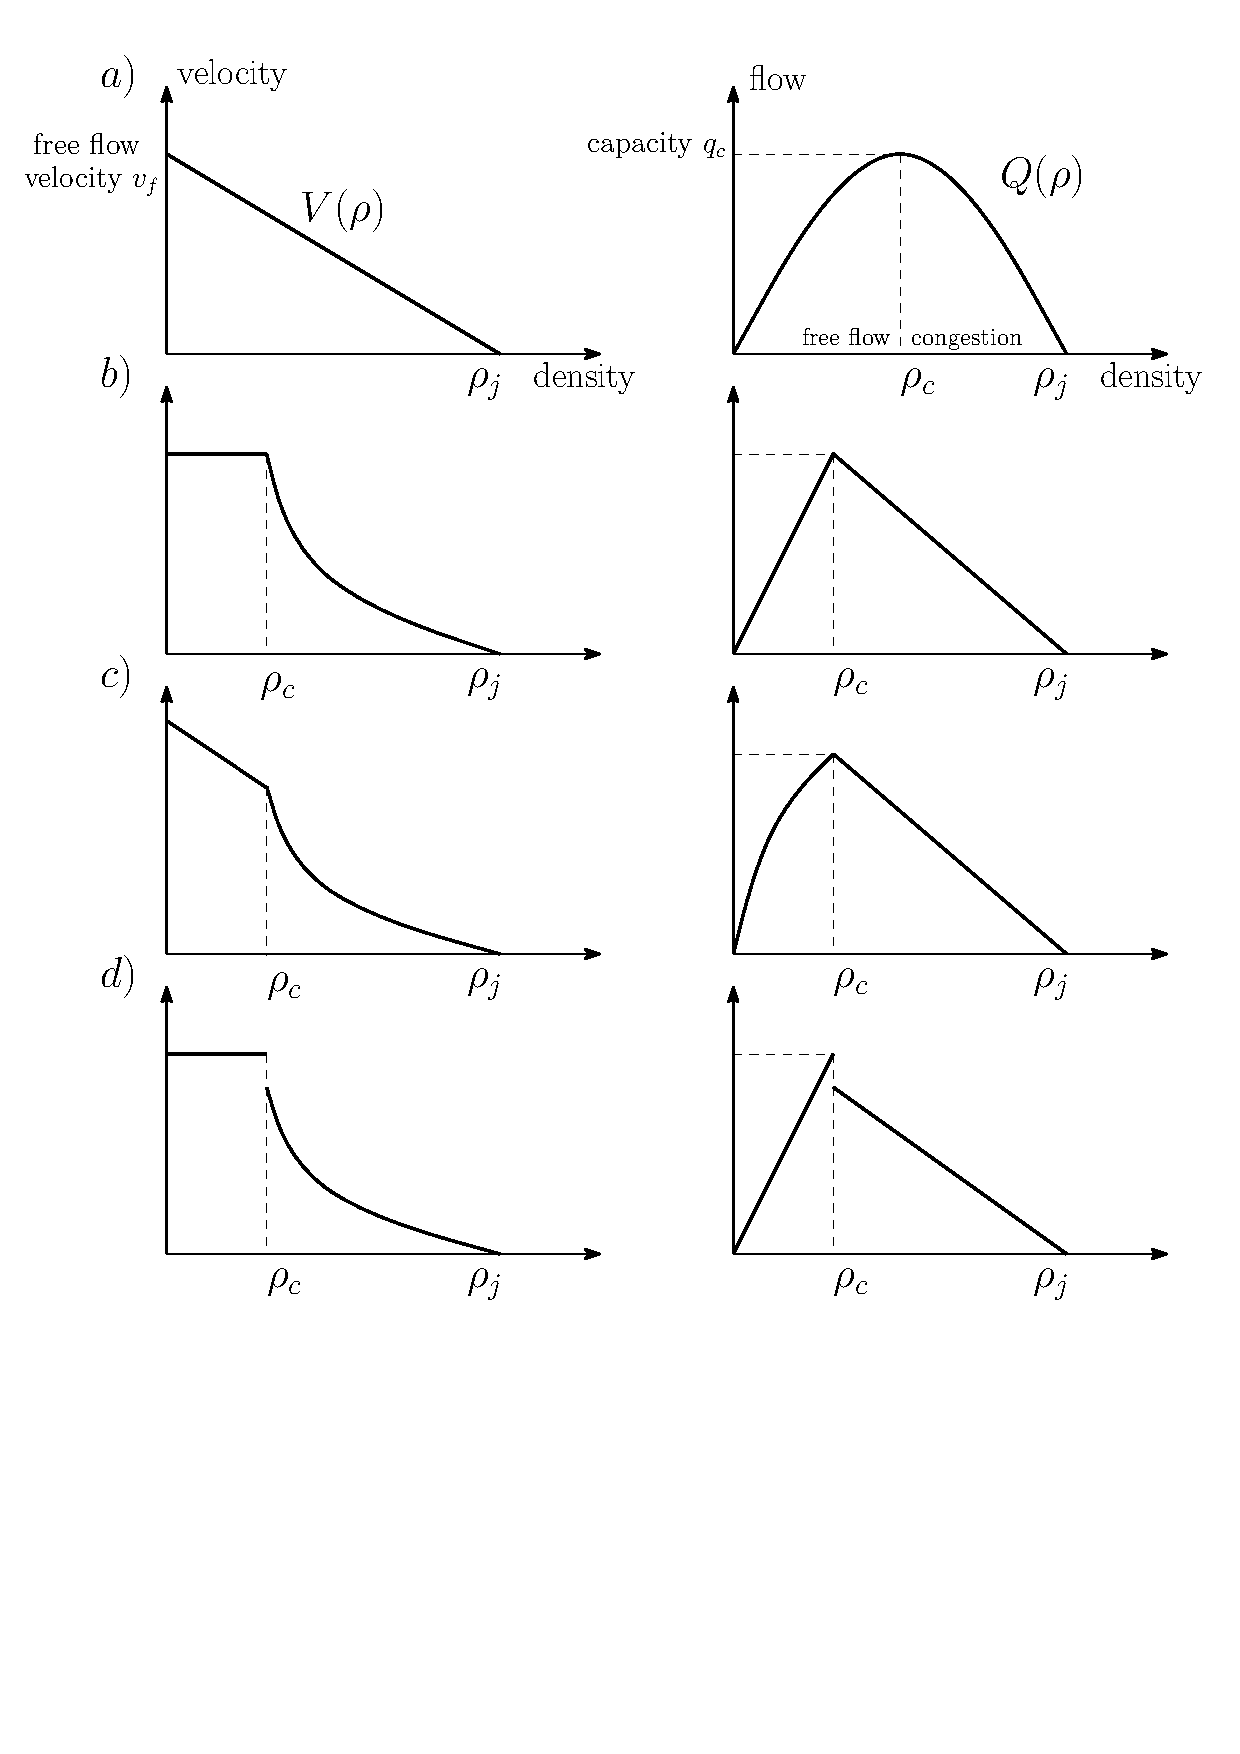
\includegraphics[width=12cm]{fundamentalDiagram.pdf}
    \caption[Common Fundamental Diagrams]{Speed and flow relationships (fundamental diagrams) for Greenshields (a), Daganzo-Newell (b), linear-hyperbolic (c), and discontinuous (d).}
\label{fig:fundamentalDiagram}
\end{figure}

\bigskip
In this project, we essentially use Greenshields and Daganzo flows. We use Greenshields for verification purposes because we can derive a complete analytical solution of the problem when using Greenshields. Daganzo is one of the most commonly and accurate fundamental that verifies concavity properties. Moreover, we have a well-calibrated Daganzo flow for the route I880 that we wish to study.

\bigskip
\noindent\underline{Greenshields flow function:} 
\begin{equation} \label{eq:greenshieldsVelocity}
v = V_{G}(\rho) = v_{f}(1-\frac{\rho}{\rho_{j}})
\end{equation}

\noindent and the corresponding flux function is:

\begin{equation} \label{eq:greenshieldsFlux}
Q_{G}(\rho) = \rho V_{G}(\rho) = v_{f}(\rho-\frac{\rho^{2}}{\rho_{j}})
\end{equation}	

\noindent\underline{Daganzo flow function:} 
\begin{equation}\label{eq:dnVelocity}
v = V_{DN}(\rho) = \left\{ \begin{array}{lcl}
v_{f} & if & \rho \leq \rho_{c} \\
-w \left( 1 - \frac{\rho_{j}}{\rho} \right) & if & \rho > \rho_{c}
\end{array}\right.
\end{equation}

\noindent and the corresponding flux function is:

\begin{equation}\label{eq:dnFlux}
Q_{DN}(\rho) = \rho V_{DN}(\rho) \left\{ \begin{array}{lcl}
v_{f} \rho & if & \rho \leq \rho_{c} \\
-w \left( \rho - \rho_{j} \right) & if & \rho > \rho_{c}
\end{array}\right.
\end{equation}

where $v_f$ is the \textit{free-flow speed}, $\rho_j$ is the \textit{jam density} (i.e $q(\rho_j)=0$), $\rho_c$ is the \textit{critical density} (i.e. \textit{free flow} when $\rho \leq \rho_{c}$ and \textit{congestion} when $\rho > \rho_{c}$) and $w$ is the backwards propagation wave speed.

\bigskip
It is important to notice that both of the previous fundamental diagrams satisfy the following properties:

(i) Hypothesis of a static flow/density relationship: $q = Q(\rho(x,t))$.

(ii) $Q(0)=Q(\rho_{j})=0$.

(iii) The continuous portions of $Q(\rho)$ are concave.

(iv) $V(0) = v_{f}$, and $V(\rho_{j}) = 0$.

(v) A critical density $\rho_{c}$ can be defined where the maximum flow $q_{c}$ is attained. Then, $Q(\rho)$ is increasing for $\rho \leq \rho_{c}$ and decreasing for $\rho > \rho_{c}$.

(vi) The critical density $\rho_{c}$ separates the fundamental diagram into two regimes: \textit{free flow} when $\rho \leq \rho_{c}$ and \textit{congestion} when $\rho > \rho_{c}$.


\subsection{Analytical solution of the LWR PDE}\label{characteristics}

The solutions of this equation can be described in terms of \textit{characteristics}, or trajectories in the time/space plane along which the densities and flows are described by ordinary differential equations. Equation (\ref{eq:LWRmodel3}) is a relatively simple wave equation: its characteristics are straight lines with slope $Q'(\rho)$. Along the characteristics, the densities and flows remain \textit{constant}. The value of the density or flow at any point is therefore equal to a boundary or initial condition to which the point is connected by a characteristic. The boundary value problem is \textit{well-posed} if the family of characteristics emanating from the initial and boundary conditions spans the entire time -space plane. The main complication arises, as described in \cite{Lighthill1955}, when characteristics intersect, leading to multiple values at the point of intersection. In this situation, the PDE admits only \textit{weak solutions}, which necessarily contain discontinuities, or \textit{shocks}. The discontinuities are such that the more general integral form of (\ref{normalLWR}) between arbitrary points $x_{1}$ and $x_{2}$ applies:

\begin{equation} \label{eq:LWRmodelIntegral}
\frac{d}{dt} \int_{x_{1}}^{x_{2}} \rho(x,t)dx + q(x_{2},t) - q(x_{1},t) = 0
\end{equation}

The speed of the shock $c_{s}$ can be found by applying (\ref{eq:LWRmodelIntegral}) to a small interval $[x_{1},x_{2}]$ containing the moving shock at $x=s(t)$ \cite{Whitham1999} (see Figure \ref{fig:speedShock}):

\begin{equation} \label{eq:csCalculus}
\begin{split}
q(x_{1},t) - q(x_{2},t) & = \frac{d}{dt}\int_{x_{1}}^{x_{2}} \rho(x,t)dx\\
& = \frac{d}{dt}\int_{x_{1}}^{s^{-}(t)}\rho(x,t)dx + \frac{d}{dt}\int_{s^{+}(t)}^{x_{2}}\rho(x,t)dx\\
& = \dot{s} \rho(s^{-},t) + \int_{x_{1}}^{s^{-}(t)}\frac{\partial \rho}{\partial t}dx - \dot{s} \rho(s^{+},t) + \int_{s^{+}(t)}^{x_{2}}\frac{\partial \rho}{\partial t}dx
\end{split}
\end{equation}

Taking the limit $x_{1} \rightarrow s^{-}$ and $x_{2} \rightarrow s^{+}$:

\begin{equation} \label{eq:speedShock}
c_{s}(t) = \dot{s}(t) = \frac{q(s^{+},t)-q(s^{-},t)}{\rho(s^{+},t)-\rho(s^{-},t)} = \frac{q^{+}-q^{-}}{\rho^{+}-\rho^{-}}
\end{equation}

This last equation, called the \textit{Rankine-Hugoniot jump condition}, gives a condition on discontinuities of weak solutions of (\ref{eq:normalLWR},\ref{eq:LWRmodel3}) relating the right and left states with the ``speed'' $c_{s}$ of the ``shock''. This last quantity is represented graphically on the fundamental diagram. This is the slope of the chord joining the upstream and downstream states, as illustrated in Figure \ref{fig:speedShock}. It is shown in \cite{Whitham1999} that the concavity of $Q(\rho)$ implies that only shocks of increasing density, or \textit{deceleration} shocks, can develop in the traffic stream. This is because conditions of heavy downstream traffic and light upstream traffic generate waves that coalesce, whereas conditions of smaller downstream density lead to diverging waves. Hence, all shocks that form naturally must satisfy:

\begin{equation} \label{eq:shocksCondition}
\rho^{-} \leq \rho^{+}
\end{equation}

\begin{figure}[here]
  \centering
    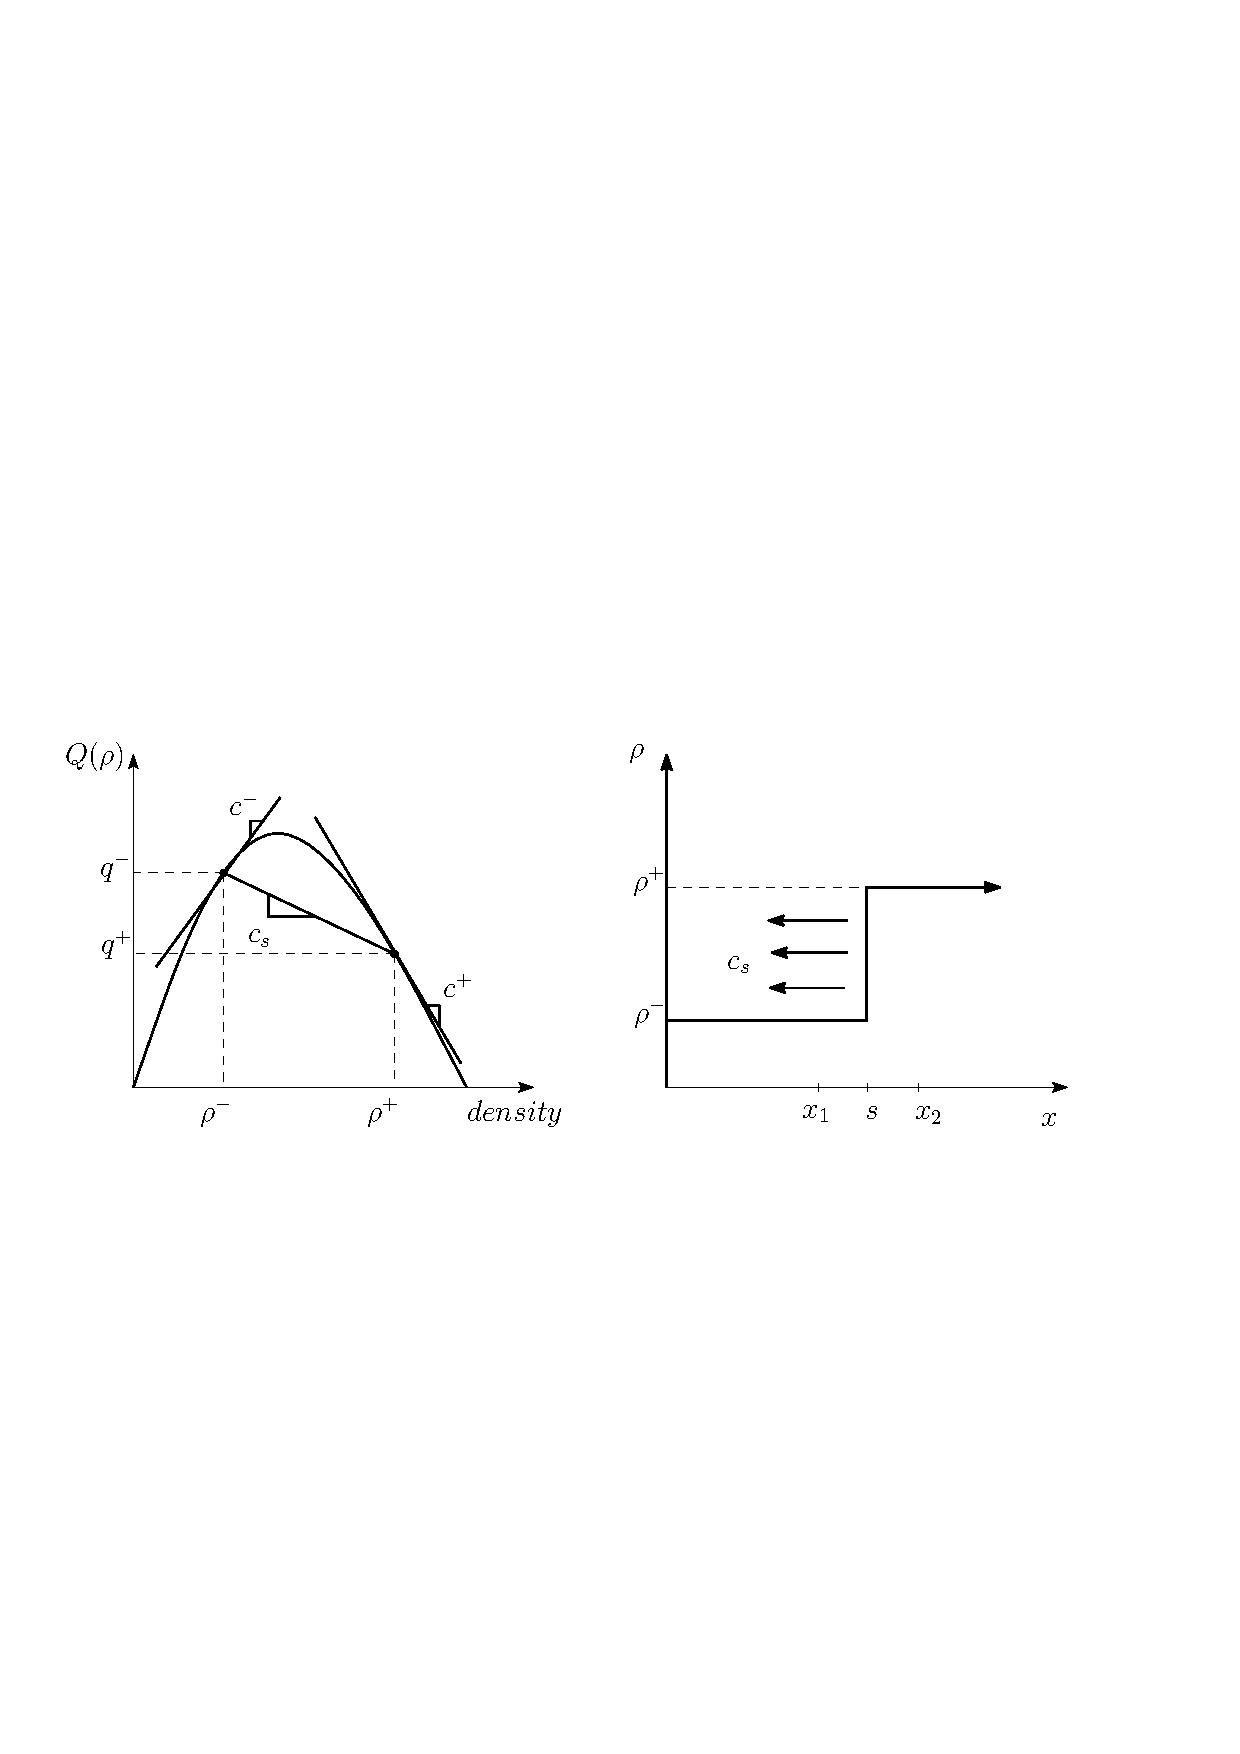
\includegraphics[width=12cm]{speed_of_shock.pdf}
    \caption{Speed of shock.}
    \label{fig:speedShock}
\end{figure}

Denoting the speed of the characteristics that terminate in the shock with $c^{-}=Q'(\rho^{-})$ and $c^{+}=Q'(\rho^{+})$, then equations (\ref{eq:speedShock}), (\ref{eq:shocksCondition}), and the concavity of $Q(\rho)$ imply:

\begin{equation} \label{eq:speedRelation}
c^{-} > c_{s} > c^{+}
\end{equation}

This condition, known as the \textit{entropy condition}, along with the \textit{jump condition} solve the problem of \textit{shock waves}. For further details on this problem, which is a specific case to the \textit{Riemann problem}, we refer the reader to \cite{Garavello2006}. We see in the next section that the \textit{Riemann problem} motivates the choice of specific mathematical schemes and algorithms when it comes to implement the models using numerical approximations.
Ansorge \cite{Ansorge1990} found in 1990 a condition of \textit{increasing entropy} that is sufficient to eliminate all of the weak solutions of LWR equation except for the physically relevant one.  This justifies why we only work with Greenshields and Daganzo flows in this project.

\subsection{The Cell Transmission Model}
A good numerical method to solve the equations along roads is represented by the Godunov scheme, which is based on exact solutions to Riemann problems \cite{Godunov1959} and the notion of entropy mentioned in Section \ref{characteristics} . This leads to the construction of a nonlinear discrete time dynamical system.

\subsubsection{Godunov Scheme}\label{godunov}

The Godunov discretization scheme is applied on the LWR PDE, where the discrete time step $\Delta T$ is indexed by $n$, and the discrete space step $\Delta X$ is indexed by $i$:

\begin{equation} \label{eq:rhoGodunov}
\rho^{n+1}_{i} = \rho^{n}_{i} - \frac{\Delta T}{\Delta X}\left(G(\rho^{n}_{i},\rho^{n}_{i+1})-G(\rho^{n}_{i-1},\rho^{n}_{i})\right)
\end{equation}

\noindent where the Godunov flux $G(\rho_{1},\rho_{2})$ is in general defined as:

\begin{equation} \label{eq:rhoGodunovFluxGeneral}
G(\rho_{1},\rho_{2}) = \left\{ \begin{array}{lll}
\text{min}_{\rho \in [\rho_{1},\rho_{2}]} Q(\rho) & \text{if} & \rho_{1} \leq \rho_{2}\\
\text{max}_{\rho \in [\rho_{2},\rho_{1}]} Q(\rho) & \text{if} & \rho_{2} \leq \rho_{1}
\end{array}\right.
\end{equation}

Similarly, we can apply the  scheme at the boundaries (see \cite{Strub2006})
\begin{equation} \label{eq:rhoGodunovleft}
\rho^{n+1}_{0} = \rho^{n}_{0} - \frac{\Delta T}{\Delta X}\left(G(\rho^{n}_{0},\rho^{n}_{1})-G(\rho^{n}_{-1},\rho^{n}_{0})\right)
\end{equation}
\begin{equation} \label{eq:rhoGodunovright}
\rho^{n+1}_{i_{max}} = \rho^{n}_{i_{max}} - \frac{\Delta T}{\Delta X}\left(G(\rho^{n}_{{i_{max}}},\rho^{n}_{{i_{max}}+1})-G(\rho^{n}_{{i_{max}}-1},\rho^{n}_{{i_{max}}})\right)
\end{equation}
\noindent with the ghost cells on the left and the right of the space interval defined as follows:
\begin{equation} \label{eq:ghostleft}
\rho^{n}_{-1} = \frac{1}{\Delta t}\int_{(n-\frac{1}{2})\Delta t}^{(n+\frac{1}{2})\Delta t} \! \rho_{a}(t) \, \mathrm{d} t.
\end{equation}
\begin{equation} \label{eq:ghostright}
\rho^{n}_{i_{max}+1} = \frac{1}{\Delta t}\int_{(n-\frac{1}{2})\Delta t}^{(n+\frac{1}{2})\Delta t} \! \rho_{b}(t) \, \mathrm{d} t.
\end{equation}
\subsubsection{CFL condition}\label{cfl}

In order to ensure numerical stability, the time and space steps are coupled by the CFL condition \cite{LeVeque1992}. In the case of our study which is a hyperbolic PDE, the CFL condition becomes:
\begin{equation}\label{eq:cfl}
\frac{\Delta T}{\Delta X} \leq \frac{1}{c_{max}}
\end{equation} 
\noindent where $c_{max}$ denotes the maximal characteristic speed.
\subsubsection{Our specific case}\label{SpecificCase}

For a family of flux functions $Q(\rho)$ sharing the same properties (i) to (vi) given in section \ref{FD}, the Godunov flux has an explicit formulation. It can also be expressed as the minimum of the \textit{sending flow} from the upstream cell and the \textit{receiving flow} from the downstream cell through a boundary connecting two cells of a homogeneous road. The \textit{sending flow} $S(\rho)$ is equal to the upstream flow if the upstream traffic is in free flow ($\rho \leq \rho_{c}$) or the capacity of the upstream section $q_{c}$ if the upstream traffic is in congestion ($\rho > \rho_{c}$); on the other hand, the \textit{receiving flow} $R(\rho)$ is equal to the capacity of the downstream section if the downstream traffic is in free flow or the downstream flow if the downstream traffic is in congestion. Notice that this explanation is related to the analytical method of characteristics highlighted in section \ref{characteristics} . The explicit formulation of the Godunov flow is given below: 
\begin{equation} \label{eq:rhoGodunovFlux1}
G(\rho_{1},\rho_{2}) = \text{min}(S(\rho_{1}),R(\rho_{2}))
\end{equation}

\begin{equation} \label{eq:sendingFlow1}
S(\rho) = \left\{ \begin{array}{lll}
Q(\rho) & \text{if} & \rho \leq \rho_{c} \\
q_{c} &  \text{if} & \rho > \rho_{c}
\end{array}\right.
\end{equation}

\begin{equation} \label{eq:receivingFlow1}
R(\rho) = \left\{ \begin{array}{lll}
q_{c} & \text{if} & \rho \leq \rho_{c} \\
Q(\rho) &  \text{if} & \rho > \rho_{c}
\end{array}\right.
\end{equation}
\noindent Or, finally,

\begin{equation} \label{eq:rhoGodunovFlux2}
G(\rho_{1},\rho_{2}) = \left\{ \begin{array}{lll}
Q(\rho_{2}) & \text{if} & \rho_{c} \leq \rho_{2} \leq \rho_{1} \\
Q(\rho_{c}) & \text{if} & \rho_{2} \leq \rho_{c} \leq \rho_{1} \\
Q(\rho_{1}) & \text{if} & \rho_{2} \leq \rho_{1} \leq \rho_{c} \\
min(Q(\rho_{1}),Q(\rho_{2})) & \text{if} & \rho_{1} \leq \rho_{2}
\end{array}\right.
\end{equation}
 In our scripts we use the formulation given by Eq.(\ref{eq:rhoGodunovFlux2}) .
 Also, for the two Fundamental Diagrams we are working with, Eq. (\ref{eq:cfl}) becomes:
 
\noindent\underline{Greenshields flow function:} 
\begin{equation}\label{eq:cfl_Gr}
\frac{\Delta T}{\Delta X} \leq \frac{1}{v_f}
\end{equation} 
 \noindent\underline{Daganzo flow function:} 
\begin{equation}\label{eq:cfl_D}
\frac{\Delta T}{\Delta X} \leq \frac{1}{\max(v_f,w)}
\end{equation} 

\subsection{Density data assimilation}
The Kalman filter operates recursively on streams of noisy input data to produce a statistically optimal estimate of the underlying system state. Based on \cite{Evensen2007}, we give here the general formulation of the Kalman Filter for discrete time systems. We explain why we can not use the 2 first approaches in this study. Finally, based on \cite{Work2010}, we give a formulation of the Ensemble Kalman Filter for the density-based model.
\subsubsection{Linear case : Kalman filter}

\noindent For a discrete-time system:
\begin{equation}\label{KF_lin}
\left\{\begin{array}{lcl} 
x(k+1) = \mathbf{M}(k)x(k) + \mathbf{B_u}(k)u(k) + \mathbf{B_w}(k)w(k)\\
y(k) = \mathbf{H}(k)x(k) + v(k)
\end{array}\right.
\end{equation}

\noindent where $v$ is the measurement noise $\mathbf{H(k)}$ the observation matrix, $u$ is the input and $w$ is the input noise, such that:
\begin{equation}\label{KF_conditions}
\left\{\begin{array}{lcl}
v(k) \sim \mathbf{N}(0,R(k))\text{ zero mean Gaussian white noise with covariance }R(k)\\
w(k) \sim \mathbf{N}(0,Q(k)) \text{ zero mean normal distribution with covariance }Q(k)\\
(x(0),w(1)...,w(k),v(1),...,v(k)) \text{are  uncorrelated}
\end{array}\right.
\end{equation}

With these assumptions, it has been shown that it is possible to compute the best estimate of $x(k)$ in the sense of least squares using a recursive algorithm by Kalman. 
\begin{itemize}\label{KF_lin_hyp}
\item Forecast step (Time-update): \begin{align}
x_{f}(k+1) & =\mathbf{M}(k)x_f(k) + \mathbf{B_u}(k)u(k)\\
\mathbf{P}_{f}^{n} &
=\mathcal{M}(k)\mathbf{P}_{a}(k)\mathcal{M}(k)^{T}
+\mathbf{Q}(k)\label{eq:kf2}\end{align}
\hspace{10 mm}
\begin{tabular}{ll}
$x_{f}(k+1)$ (resp. $x_{a}(k+1)$) &: forecast (analyzed) state estimate\\
\end{tabular}\\

\item Analysis step (Measurement-update): \begin{align}
x_{a}(k+1) &
=x_{f}(k+1)+\mathbf{G}(k+1)\left(y(k+1)-\mathbf{H}(k+1)x_{f}(k+1)\right)\\
\mathbf{P}_{a}(k+1)&
=\mathbf{P}_{f}(k+1)-\mathbf{G}(k+1)\mathbf{H}(k+1)\mathbf{P}_{f}(k+1)\\
\mathbf{G}(k+1) &
=\mathbf{P}_{f}(k+1)\mathbf{H}(k+1)^{T}\left(\mathbf{H}(k+1)\mathbf{P}
_{f}(k+1)\mathbf{H}(k+1)^{T}+\mathbf{R}(k+1)\right)^{-1}\label{
eq:kalmangain}\end{align}

$\mathbf{P}_{f}(k+1)$ (resp. $\mathbf{P}_{a}(k+1)$) : error covariance of the forecast (analyzed) state

\end{itemize} 

\subsubsection{Extended Kalman filter}\label{Ext_Kal_v}
In our case we are working with an autonomous equation, i.e. without input, so we can simplify the equations. We now apply every formula found in literature for our specific application. We process by analogy with what was done in \cite{} with a velocity formulation of the problem. If equation~\eqref{eq:rhoGodunov} was differentiable in $\rho^{n}$,
so would be the operator $\mathcal{M}[\cdot]$ in~\eqref{eq:ekf1},
in which case the optimal estimate for the state $\rho^{n}$ could be
obtained using the traditional Extended Kalman Filter
equations. These are simply the Jacobian linearized version of the linear case.

\begin{itemize}
\item Forecast step (Time-update): \begin{align}
\rho_{f}^{n} & =\mathcal{M}(\rho_{a}^{n-1})\label{eq:ekf1}\\
\mathbf{P}_{f}^{n} &
=\mathcal{M}_{L}^{n-1}\mathbf{P}_{a}^{n-1}\left(\mathcal{M}_{L}^{n-1}\right)^{T}
+\mathbf{Q}^{n-1}\label{eq:ekf2}\end{align}
\hspace{10 mm}
\begin{tabular}{ll}
${\rho}_{f}^{n}$ (resp. ${\rho}_{a}^{n}$) &: forecast (analyzed) state estimate\\
$\mathcal{M}_{L}^{n}=\frac{\partial\mathcal{M}(\rho_{a}^{n})}{\partial \rho_{a}^{n}}$& : jacobian matrix of $\mathcal{M}$\\
\end{tabular}\\


\item Analysis step (Measurement-update): \begin{align}
\rho_{a}^{n} &
=\rho_{f}^{n}+\mathbf{G}^{n}\left(y^{n}-\mathbf{H}^{n}\rho_{f}^{n}\right)\\
\mathbf{P}_{a}^{n} &
=\mathbf{P}_{f}^{n}-\mathbf{G}^{n}\mathbf{H}^{n}\mathbf{P}_{f}^{n}\\
\mathbf{G}^{n} &
=\mathbf{P}_{f}^{n}\left(\mathbf{H}^{n}\right)^{T}\left(\mathbf{H}^{n}\mathbf{P}
_{f}^{n}\left(\mathbf{H}^{n}\right)^{T}+\mathbf{R}^{n}\right)^{-1}\label{
eq:kalmangain}\end{align}

$\mathbf{P}_{f}^{n}$ (resp. $\mathbf{P}_{a}^{n}$) : error covariance of the forecast (analyzed) state

\end{itemize} 


\subsubsection{Ensemble Kalman filter}
As mentioned in section \ref{Ext_Kal_v}, the Extended Kalman filter implementation requires the equation governing the density evolution to be differentiable whereas, in the case of the discretized LWR equation using Godunov scheme, it is not. Indeed, nondifferentiability comes from both the Godunov scheme itself (see $\min (.)$) and the flow function (see Daganzo in (\ref{eq:dnFlux})). In this case there is no easy way to compute the error covariance matrices in a recursive way as in sections \ref{KF_lin} and \ref{Ext_Kal_v}. To make up for this impossibility, the apriori error covariance is computed by a Monte-Carlo type of approach reasoning on an ensemble of values of $\rho^n$ instead of one averaged value.  
Finally, the ensemble Kalman filter algorithm can be summarized as follows \cite{Evensen2007}:

\begin{center}
\framebox{\begin{minipage}[t]{0.95\columnwidth}
\begin{enumerate}
\item \emph{Initialization}:  Draw $K$ ensemble realizations $\rho_{a}^{0}(k)$
(with $k\in\{1,\cdots,K\}$) from a process with a mean speed $\bar{\rho}_{a}^{0}$
and covariance $\mathbf{P}_{a}^{0}$. 
\item \emph{Forecast}: Update each of the $K$ ensemble members according
to the Godunov discretization scheme. Then update the ensemble mean and covariance according to: 
\begin{align}
\rho_{f}^{n}(k) & =\mathcal{M}(\rho_{a}^{n-1}(k))+\eta^{n}(k)\label{eq:enkf1}\\
\bar{\rho}_{f}^{n} & =\frac{1}{K}\sum_{k=1}^{K}\rho_{f}^{n}(k)\label{eq:enkf2}\\
\mathbf{P}_{\text{ens},f}^{n} &
=\frac{1}{K-1}\sum_{k=1}^{K}\left({\rho}_{f}^{n}(k)-\bar{\rho}_{f}^{n}\right)\left({\rho}
_{f}^{n}(k)-\bar{\rho}_{f}^{n}\right)^{T}\label{eq:enkf3}\end{align}

\item \emph{Analysis}: Obtain measurements, compute the Kalman gain, and
update the network forecast: 
\begin{align}
\mathbf{G}_{\text{ens}}^{n} &
=\mathbf{P}_{\text{ens},f}^{n}\left(\mathbf{H}^{n}\right)^{T}\left(\mathbf{H}^{n
}\mathbf{P}_{\text{ens},f}^{n}\left(\mathbf{H}^{n}\right)^{T}+\mathbf{R}^{n}
\right)^{-1}\label{eq:enkf4}\\
\rho_{a}^{n}(k) &
=\rho_{f}^{n}(k)+\mathbf{G}_{\text{ens}}^{n}\left(y^n(k)-\mathbf{H}^{n
}\rho_{f}^{n}(k)+\chi^{n}(k)\right)\label{eq:enkf5}\end{align}

\item Return to 2. 
\end{enumerate}
\end{minipage}}

\par\end{center}
\noindent where $\mathcal{M(.)}$ is the Godunov operator, $\chi^{n}$ is the measurement noise, $\eta^{n}$ the state noise and $y^{n}$ the measurements.
\subsection{Extension to networks}

Even though we did not have time to implement the density-based model on a road network, we present here the theory that will enable us to do it in the future. The road network is represented by a directed graph consisting of vertices $v \in \mathcal{V}$, which represent the junctions in the network, and edges $e \in \mathcal{E}$, which are the links. Each link $e$ is divided into cells numbered from $0$ to $I_{e}$, which gives the density fields for the entire network $\rho^{n}=\rho^{n}_{i,e}, {e\in \mathcal{E}, i=0,...,I_{e}}$, at each time step. For two consecutive cells without any junction the evolution of the density field is governed by the same equations as before.

\bigskip
Let us consider a junction $v$ with $\mathcal{I}(v)$ and $\mathcal{O}(v)$ the sets of incoming and outgoing edges respectively and assume that the traffic entering from an incoming edge is distributed amongst the outgoing edges according to an allocation matrix $A_{v}=(\alpha^{v}_{e,e'})$ where $e \in \mathcal{I}(v)$, and $e' \in \mathcal{O}(v)$. For all the vehicles entering the junction $v$ on edge $e$, $\alpha^{v}_{e,e'}$ denotes the proportion of vehicles which will exit the junction through edge $e'$. We note that $\displaystyle\sum\limits_{e'\in \mathcal{O}(v)} \alpha^{v}_{e,e'} = 1$ for any $e\in \mathcal{I}(v)$, and the conservation of flux gives $\displaystyle\sum\limits_{e\in \mathcal{I}(v)} \alpha^{v}_{e,e'} Q_{e} = Q_{e'}$ for any $e' \in \mathcal{O}(v)$. But strong boundary conditions (i.e. equality) cannot always be imposed for an arbitrary pair ($\displaystyle\sum\limits_{e\in \mathcal{I}(v)} \alpha^{v}_{e,e'} Q_{e},\quad Q_{e'})$, so the boundary conditions provide upper bounds on the admissible incoming and admissible outgoing fluxes over which the flow through the incoming edges is maximized:

\begin{equation}\label{eq:rhoJunctionLP}
\begin{array}{rl}
\text{maximize } & 1^{T}\xi \\
\text{s.t. } & A_{v}\xi\leq \delta_{\mathcal{O}(v)} \\
& 0 \leq \xi \leq \delta_{\mathcal{I}(v)}
\end{array}
\end{equation}

\noindent where $\delta_{\mathcal{I}(v)} = (\delta_{e})_{e \in \mathcal{I}(v)}$, $\delta_{\mathcal{O}(v)} = (\delta_{e'})_{e' \in \mathcal{O}(v)}$ are the upper bounds on the edges entering and exiting the junction respectively. In the discrete case, they are given by:

\begin{equation}\label{eq:rhoUpperBound1}
\delta_{e} = Q(\rho^{n}_{I_{e},e}) \text{ for any } e \in \mathcal{I}(v)
\end{equation}

\begin{equation}\label{eq:rhoUpperBound2}
\delta_{e'} = Q(\rho^{n}_{0,e'}) \text{ for any } e' \in \mathcal{O}(v)
\end{equation}

\noindent With the optimal solution to (\ref{eq:rhoJunctionLP}), denoted by $\xi^{*}$, we can update $G(\rho^{n}_{-1,e'},\rho^{n}_{0,e'})$ and $G(\rho^{n}_{I_{e},e},\rho^{n}_{I_{e}+1,e})$ through:

\begin{equation}\label{eq:rhoUpdateBound1}
G(\rho^{n}_{I_{e},e},\rho^{n}_{I_{e}+1,e}) = \xi^{*}_{e} \text{ for any } e \in \mathcal{I}(v)
\end{equation}

\begin{equation}\label{eq:rhoUpdateBound2}
G(\rho^{n}_{-1,e'},\rho^{n}_{0,e'}) = \displaystyle\sum\limits_{e\in \mathcal{I}(v)} \alpha^{v}_{e,e'} \xi^{*}_{e} \text{ for any } e' \in \mathcal{O}(v)
\end{equation}

\newpage
\section{Implementation}

\subsection{Density measurements}
Single-loop detector data with a sample period of $30$ seconds is used
as a source of measurements for the density-based highway
model.

Single-loop sensors are essentially metal detectors which measure
the flow of traffic by counting the number of vehicles having crossed
them during a fixed period of time (hereby referred to as the loop
detector's sample period); an indirect measure of density is also
obtained by recording the percentage of time during which the detector
was occupied by a vehicle (known as the occupancy of the sensor for
the sample period).

Due to their low cost and their relative simplicity, loop
detectors constitute the single most abundant source of traffic
data. Loop detectors are grouped into stations; the measurements of
the sensors at each station are sent periodically for data
processing. Typically, each station will describe a single ``point''
of the highway and will thus have as many sensors as the number of
lanes at the highway location considered.

The following pre-processing steps are necessary in order to make the
single-loop detector data suitable for use by the density-based
highway model:
\begin{itemize}
\item Converting the occupancy measurements to
  spatial densities by using an estimate of the average effective
  vehicle length (or the g-factor)
\item Raw occupancy data is noisy and is filtered using
  heuristics which determine the quality of a datum. Bad data is
  discarded, which results occasionally in ``holes'' in the measurements.
\item Finally, each loop detector station describes
  traffic on the different lanes of the highway: in order to obtain a
  single-pipe measurement for each  time sample and each station, the
  multi-lane densities are summed.
\end{itemize}

\subsection{Constructing the EnKF observation matrix}
In its current state, the density-based highway model can only be run
on routes. Routes in this report are defined as straight-line
stretches of road along the highway going in a single direction; they
are devoid of ramps, traffic signals, toll booths, or any of the
real-life disturbances which normally affect highway traffic.
The data structures used to describe the topology of the highway in
the \emph{Mobile Millennium} codebase have been leveraged : routes
are composed of Model Graph links going in the same direction (model
graph links have a pre-defined length). For the highway model to work
correctly, it is imperative that the links be provided in the correct
geographical order. The links are then divided into $m$ cells of
length $l$. Care should be taken when segmenting the route into cells
to ensure that the CFL condition is not broken. The link information
(link ID, number of cells, cell length) is stored in a MATLAB struct.

The locations of the loop detector stations along the highway are
retrieved from the \emph{MM} database in terms of model graph links
and offsets. From this information, it becomes possible to determine
which cells contain sensors. Furthermore, the ``deceased'' sensor
stations (i.e. stations showing no sign of activity for the entire
period of time considered) are discarded. The sensor information is
stored in a separate MATLAB struct. The density measurements for the
sensors under consideration are then retrieved. 

Finally, because loop detector stations do not always report
measurements, it is necessary to build a sensor activity vector of
size $1 \times m$ at each iteration of the EnKF: if a sensor in cell
$i$ is active (inactive) at timestep $j$, then the $j$th sensor activity vector will have a value of one (zero) in its $i$th position.

For a route with $m$ cells, the observation matrix $H_j$ at each
timestep $j$ is constructed in the following way using the collected
data:
\begin{enumerate}
  \item Using the sensor information and the link information, a
    static $H$ matrix is built: cells containing a sensor have a value
    of one in the matrix, whereas cells without a sensor have a value
    of 0.
  \item At each iteration $j$ of the EnKF, a matrix $H_j$ is formed by
    multiplying $H$ by the corresponding sensor activity column
    vector: the inactive sensors at timestep $j$ are effectively
    ``zeroed out''.
\end{enumerate}

\subsection{Initialization}
The following parameters are used in the density based highway model:
\begin{itemize}
  \item The free-flow velocity and the jam density are set to default values
  \item The boundary conditions and the initial conditions are set to $0$
  \item The initial ensemble has a zero-mean multivariate normal distribution, with a covariance matrix scaled by $(\frac{\rho_{jam}}{2})^{2}$. 
  \item The state noise has a zero-mean multivariate normal distribution with a covariance matrix scaled by $(\frac{\rho_{jam}}{2})^{2}$. The noise amplitude can be adjusted. The noise is constant at each time step $j$.
  \item The measurement noise has a zero-mean multivariate normal distribution with a covariance matrix $R_j$ at timestep $j$.
\end{itemize}

\subsection{Description of the main algorithm}

As the cells do not have the same length, we choose to fix $\Delta t$ to verify the CFL condition for stability of the Godunov numerical scheme for the minimum cell length. Therefore, in the case of a Greenshields flow, we have :
\begin{equation}\label{cfl_var_cell}
\Delta t \leq \frac{\min(\Delta x )}{v}
\end{equation}

To be more accurate, we fix $\Delta t$ to a value inferior to the one given by Eq. (\ref{cfl_var_cell}) and that divides the time step for which we have measurements. In our specific study, it turns out that we get measurements every 30 seconds and that $\Delta t = 5$ seconds verifies Eq. (\ref{cfl_var_cell}). Therefore, we can represent the algorithm we implement by the flow chart on Figure \ref{main_algo}.
\begin{figure}
\centering
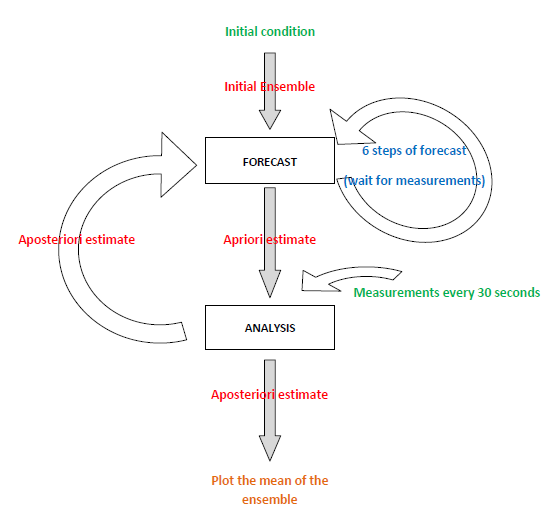
\includegraphics[width=10cm]{figures/main_algo.png}
\caption{Flow chart describing the main algorithm}
\label{main_algo}
\end{figure}


\newpage
\section{Analytical Results}
\subsection{Verification of the CTM script}\label{verif_ctm}

\paragraph{Problem description and analytical solution}\label{analytical}
In section (\ref{characteristics}), we explained how to deal with the Riemann problem analytically. Here, we derive the analytical solution of a well-posed problem so as to use it as a reference to verify our implementation of the algorithms described previously. Our next simulations were done over 100  [units of time]. The full problem for which we derived solution is the following:

\begin{equation}
\left\{\begin{array}{lcl}\label{analytical_pb}
	\rho_t + q'(\rho)\rho_x = 0\\
	q(\rho) = v \rho(1- \frac{\rho}{\rho_{max}})\\
\end{array}
\right.
\end{equation}
\noindent with, for the simulation, $v=1$ and $\rho_{max}=4$.

\noindent with the initial conditions : 
\begin{equation}
\left\{\begin{array}{lcl}\label{analytical_pb_bc_ic}
	\rho(x,0) = 1 & \text{if} & x \leq  0 \\
	\rho(x,0) = 1+x & \text{if} & x \in [0,1] \\
	\rho(x,0) = 2 & \text{if} & x \in [1,10] \\
	\rho(x,0) = 2+2(x-10) & \text{if} & x \in [10,11] \\
	\rho(x,0) = 4 & \text{if} & x \in [11,20] \\
	\rho(x,0) = 1 & \text{if} & x \geq 20 \\
\end{array}\right.
\end{equation}

In this particular case, the problem is well-posed because the analytical approach enables to work on an infinite space domain. Therefore, the characteristics span the whole time-space plane.  After deriving all the equations of the characteristics, shocks and expansion waves, we reach the following closed form of the solution:

\begin{equation}
\left\{\begin{array}{lcl}\label{analytical_pb_sol}
	\rho(x,0) = 1 & & \forall (x,t) \in  abACDE \\
	\rho(x,0) = \frac{1+x-vt}{1-\frac{vt}{2}} & & \forall (x,t) \in  bAc \\
	\rho(x,0) = 2 & & \forall (x,t) \in  cACBd \\
	\rho(x,0) = 2(1+\frac{x-10}{1-vt}) & & \forall (x,t) \in  dBE \\
	\rho(x,0) = 4 & & \forall (x,t) \in  eBCDf \\
	\rho(x,0) = 2(1-\frac{x-20}{vt}) & & \forall (x,t) \in  EDfF \\
	\rho(x,0) = 1 & & \forall (x,t) \in  Ffg\\
\end{array}\right.
\end{equation}

The plot of this solution is shown on Figure \ref{analytical_solution_plot}.

\begin{figure}
\centering
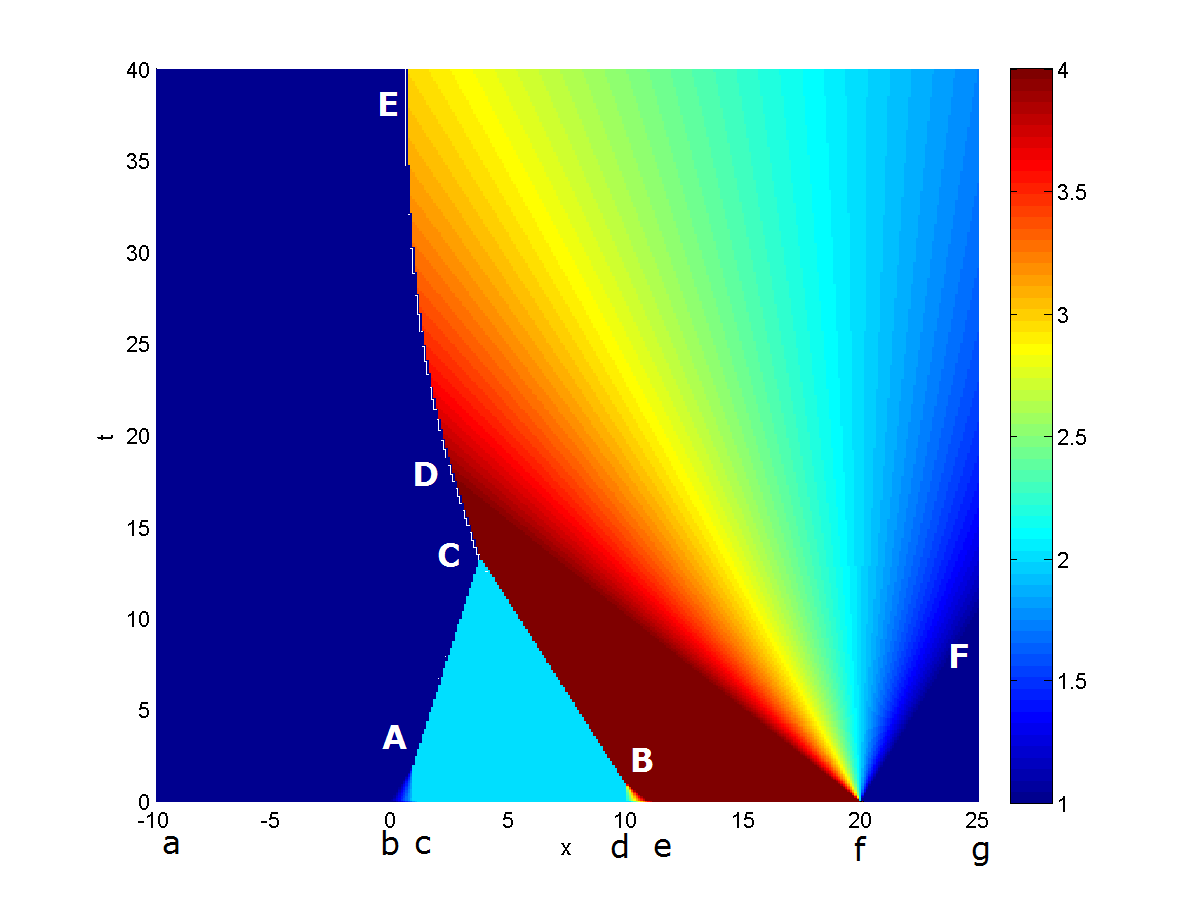
\includegraphics[width=10cm]{../Simulation_Results/Verify_CTM_results/Analytical.png}\\
    \caption{Analytical solution of the Riemann problem given by Eq.(\ref{analytical_pb}) and (\ref{analytical_pb_bc_ic})}
    \label{analytical_solution_plot}
\end{figure}

\paragraph{Numerical solution}

\begin{figure}
  \centering
  \subfloat[time-space plot]{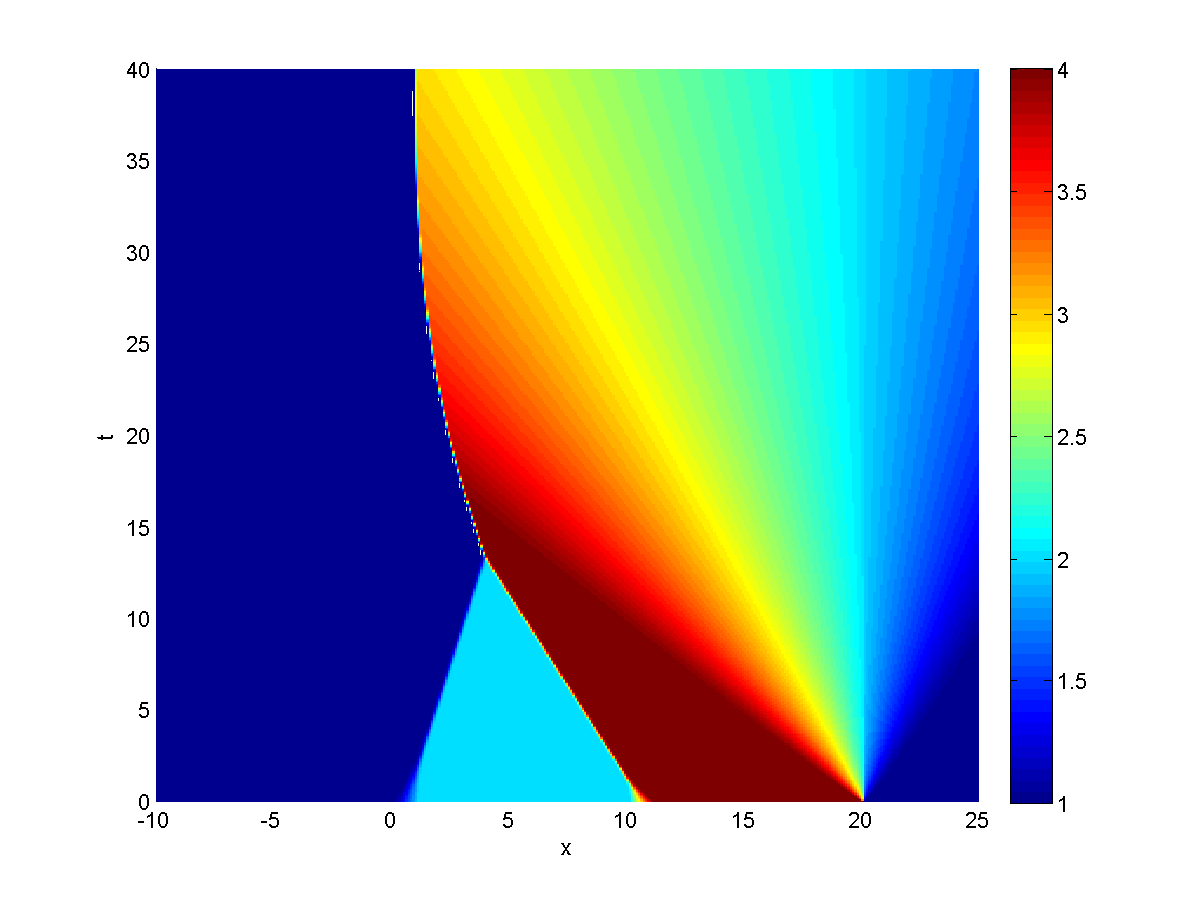
\includegraphics[width = 7cm]{../Simulation_Results/Verify_CTM_results/Numerical.png}}                
  \subfloat[3D plot]{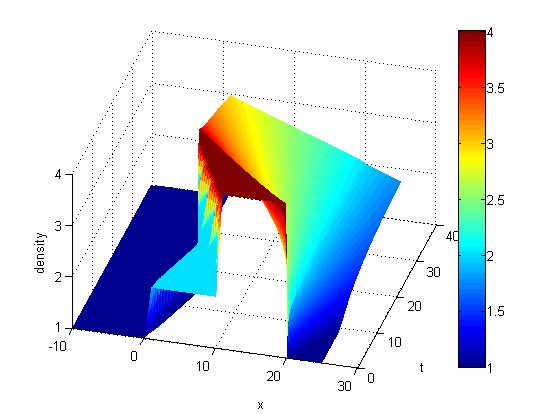
\includegraphics[width = 7cm]{../Simulation_Results/Verify_CTM_results/Numerical_3D.png}}
  \caption{Numerical results for the Riemann problem given by Eq.(\ref{analytical_pb}) and (\ref{analytical_pb_bc_ic})}
  \label{Numerical_Sol}
\end{figure}

\bigskip
From Figure \ref{Numerical_Sol} , we can ensure that the initial condition propagates correctly with the numerical scheme we used. Indeed, the shocks and zone of expansion waves clearly appear. To have a better idea on how the numerical scheme performs, we plot the difference of the numerical and the analytical result on Figure \ref{Numerical_err} .

\begin{figure}
  \centering
  \subfloat[time-space plot]{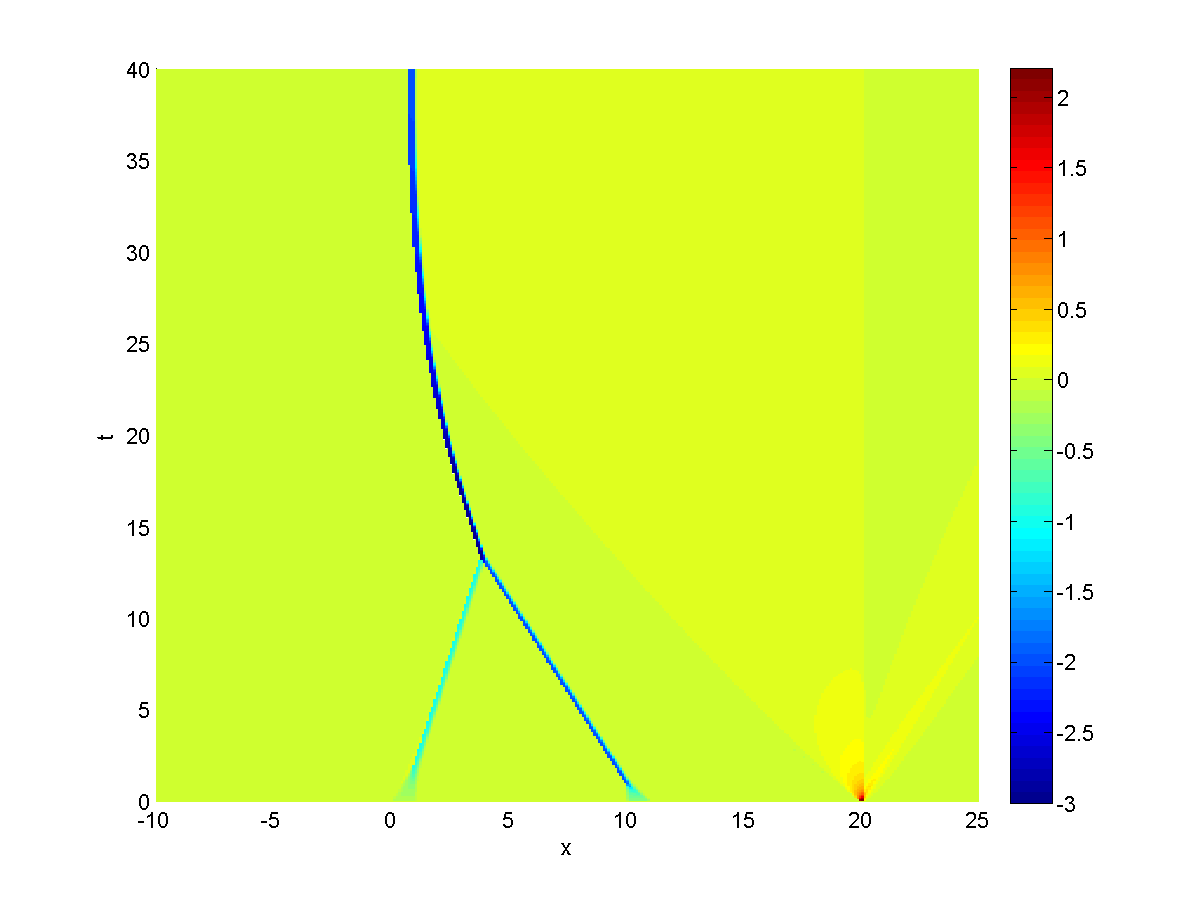
\includegraphics[width = 7cm]{../Simulation_Results/Verify_CTM_results/Error.png}}                
  \subfloat[3D plot]{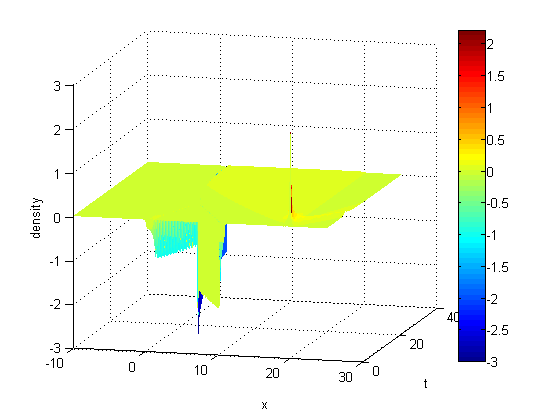
\includegraphics[width = 7cm]{../Simulation_Results/Verify_CTM_results/Error_3D.png}}
  \caption{Numerical error of the $\rho-$CTM model for the Riemann problem given by Eq.(\ref{analytical_pb}) and (\ref{analytical_pb_bc_ic})}
  \label{Numerical_err}
\end{figure}

\bigskip
We notice from these plots that the numerical solution almost perfectly matches with the analytical approach. The only areas of significant error are the areas of the time-space domain where the shocks occur. Indeed, the analytical solution has 'infinite slope' (discontinuity in $\rho$) which cannot be achieved by the numerical scheme. Then, the result obtained is very satisfying. All the more as this simulation was run with an '$r$' parameter of the Godunov scheme close to the limit value defined by the CFL condition. (see (\ref{cfl}))

\paragraph{Verification of the CTM for Daganzo flow:}
In our script, we use an overloaded function \textit{rho\_CTM} that executes the CTM for the LWR equation with either Greenshields flow or Daganzo. Figures \ref{Daganzo_test1} and \ref{Daganzo_test2} show the numerical solutions for different values of critical density for a Daganzo flow. The other values ($v$ and $\rho_{max}$) are common with the other simulations.

\begin{figure}
  \centering
  \subfloat[time-space plot]{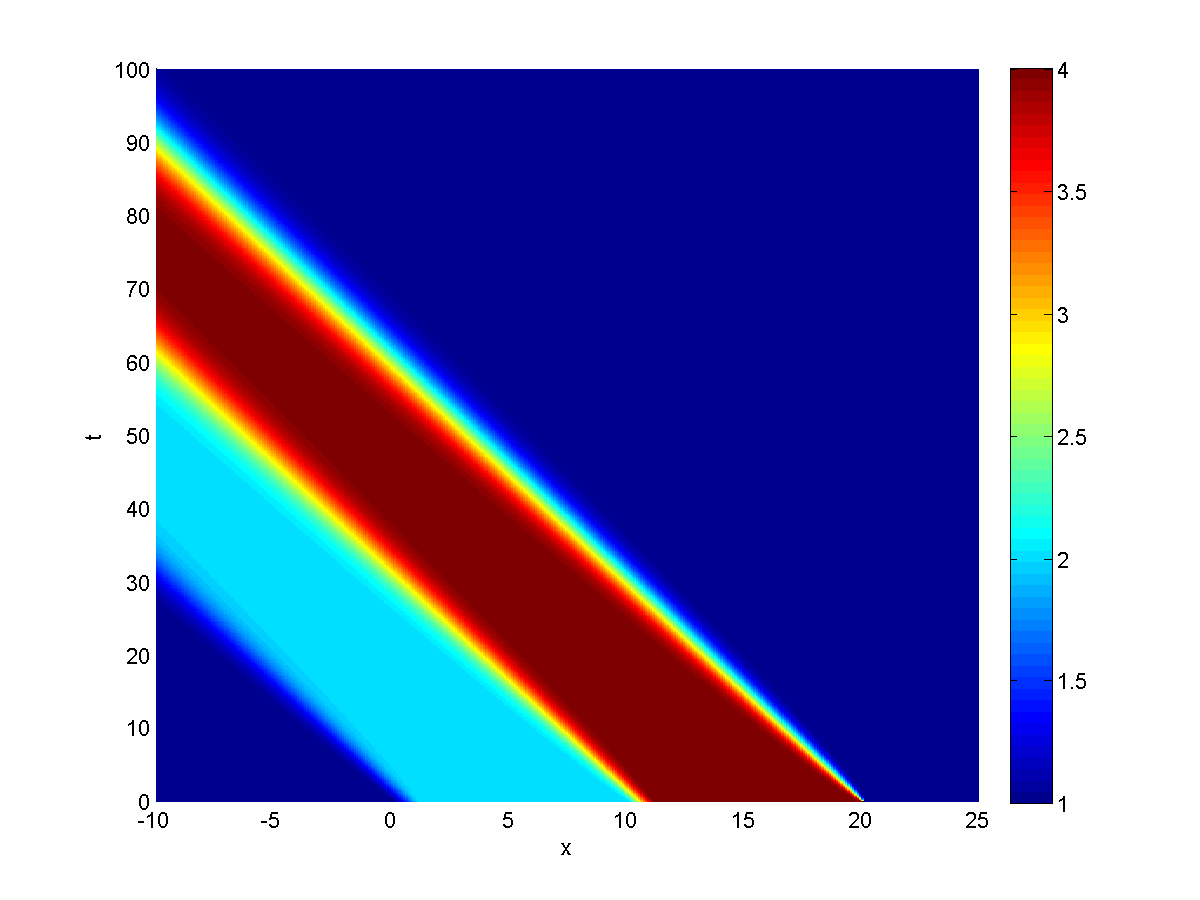
\includegraphics[width = 7cm]{../Simulation_Results/Test_CTM_daganzo/Test_Daganzo1.png}}                
  \subfloat[3D plot]{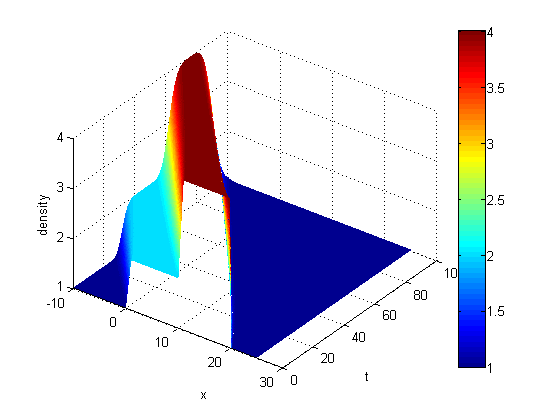
\includegraphics[width = 7cm]{../Simulation_Results/Test_CTM_daganzo/Test_Daganzo1_3D.png}}
  \caption{Propagation of the initial condition  Eq.(\ref{analytical_pb_bc_ic}) with Daganzo flow for $\rho_c=1$.}\label{Daganzo_test1}
\end{figure}

\begin{figure}
  \centering
  \subfloat[time-space plot]{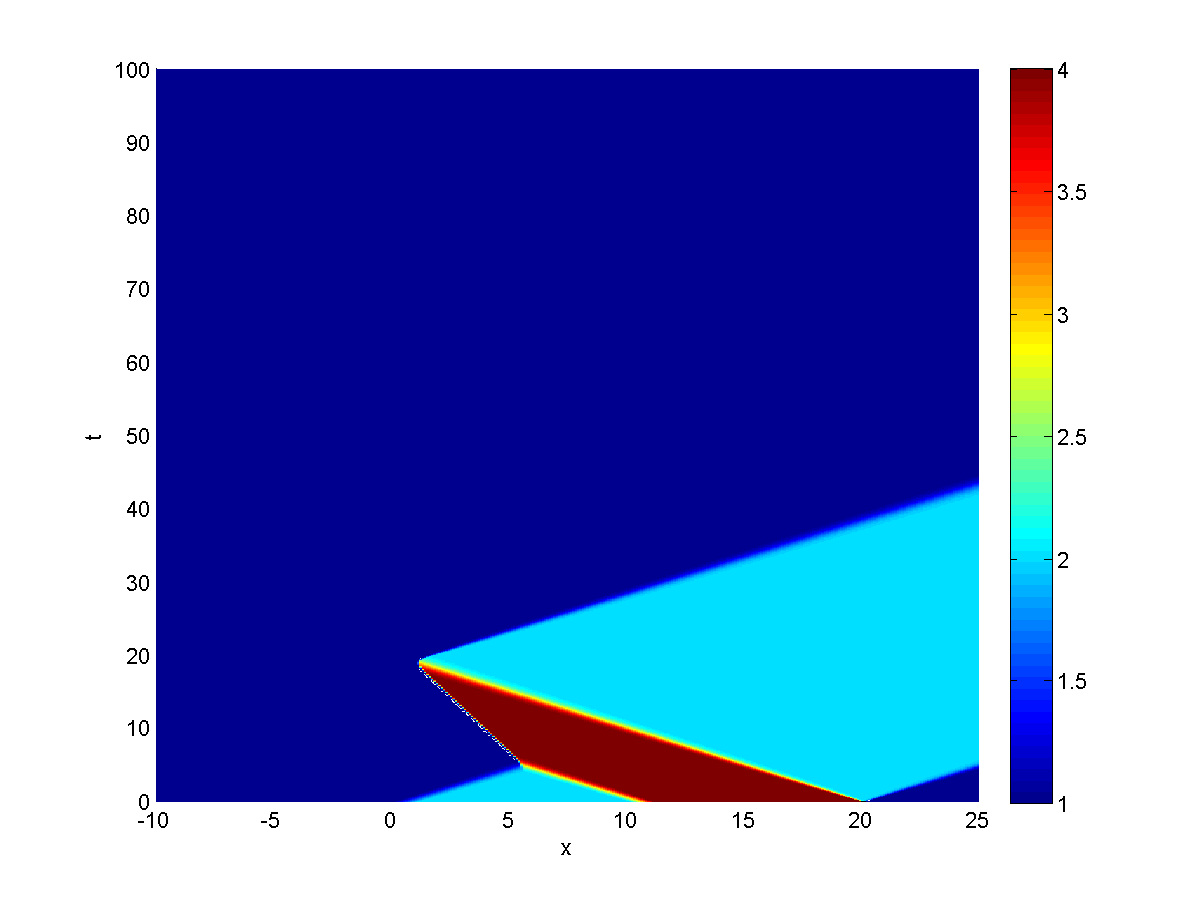
\includegraphics[width = 7cm]{../Simulation_Results/Test_CTM_daganzo/Test_Daganzo2.png}}                
  \subfloat[3D plot]{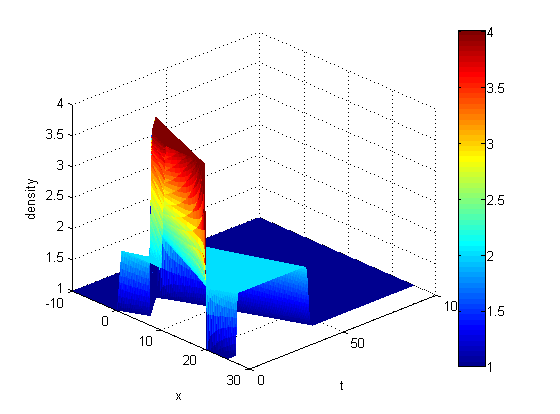
\includegraphics[width = 7cm]{../Simulation_Results/Test_CTM_daganzo/Test_Daganzo2_3D.png}}
  \caption{Propagation of the initial condition  Eq.(\ref{analytical_pb_bc_ic}) with Daganzo flow for $\rho_c=2$.}\label{Daganzo_test2}
\end{figure}

From this test, we can conclude that the overloading of the function \textit{rho\_CTM} in our code performs well for both Daganzo and Greenshields.

\subsection{EnKF-implementation verification}
Once our $\rho$ -CTM implementation proves to be efficient, we can test our implementation of the EnKF and vary some parameters (state noise, initial covariance of the ensemble, initial guess, number of steps) so as to identify their respective influence. In this part, we will use the analytical solution as both measurements and reference to check that the EnKF converges to the analytical solution. So as to make the study more interesting, we will also vary the number of cells in which we have a sensor and the frequency at which we get measurements. 

\bigskip
\paragraph{Influence of the state noise: }
Figures \ref{influence_stateNoise1}, \ref{influence_stateNoise2} and \ref{influence_stateNoise3} show the influence of the state noise on the result. In this case, the percentage of cells which have a sensor is 20\%, we have measurements 20\% of the time steps, and, the measurement noise and the initial ensemble both have a '5\% amplitude'. We simulated for a state noise of 1\%, 5\% and 10\%. (All percentages are standard deviation)

\begin{figure}
  \centering
  \subfloat[time-space plot]{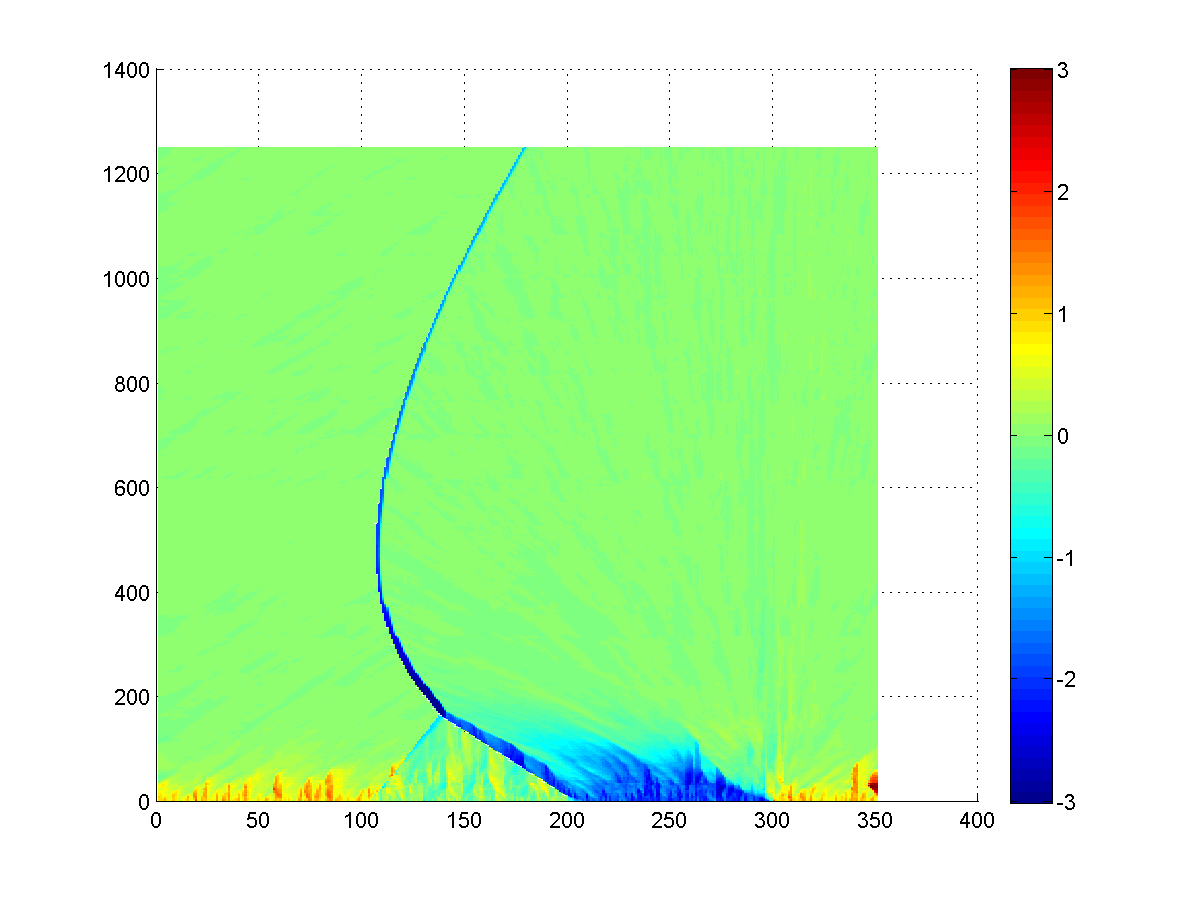
\includegraphics[width = 6cm]{../Simulation_Results/Test_EnKF/Fixed_steps_and_noise_meas_in_stateN_01.png}}
  \subfloat[3D plot]{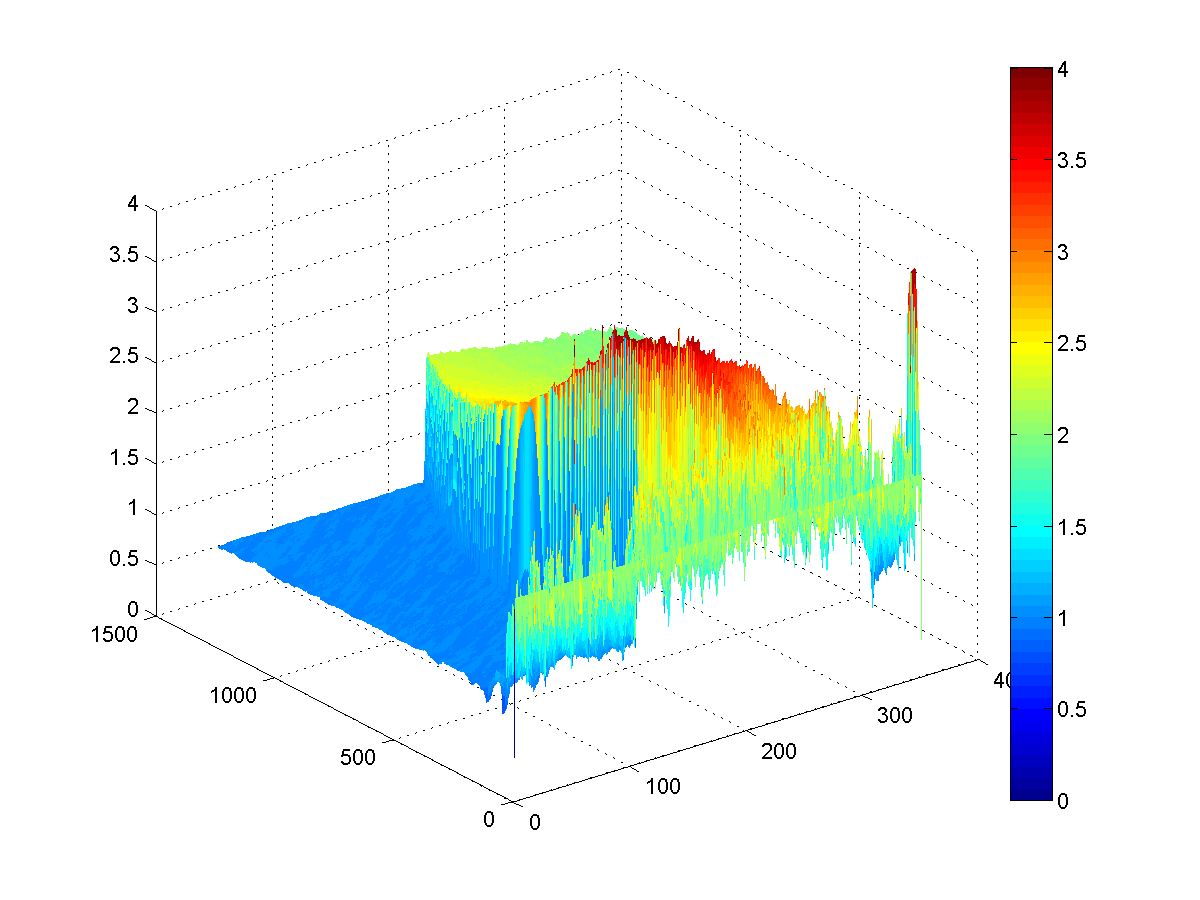
\includegraphics[width = 6cm]{../Simulation_Results/Test_EnKF/Fixed_steps_and_noise_meas_in_stateN_01_3D.png}}
  \caption{Test EnKF, influence of the state noise : 1\%}\label{influence_stateNoise1}
\end{figure}

\begin{figure}
  \centering
   \subfloat[time-space plot]{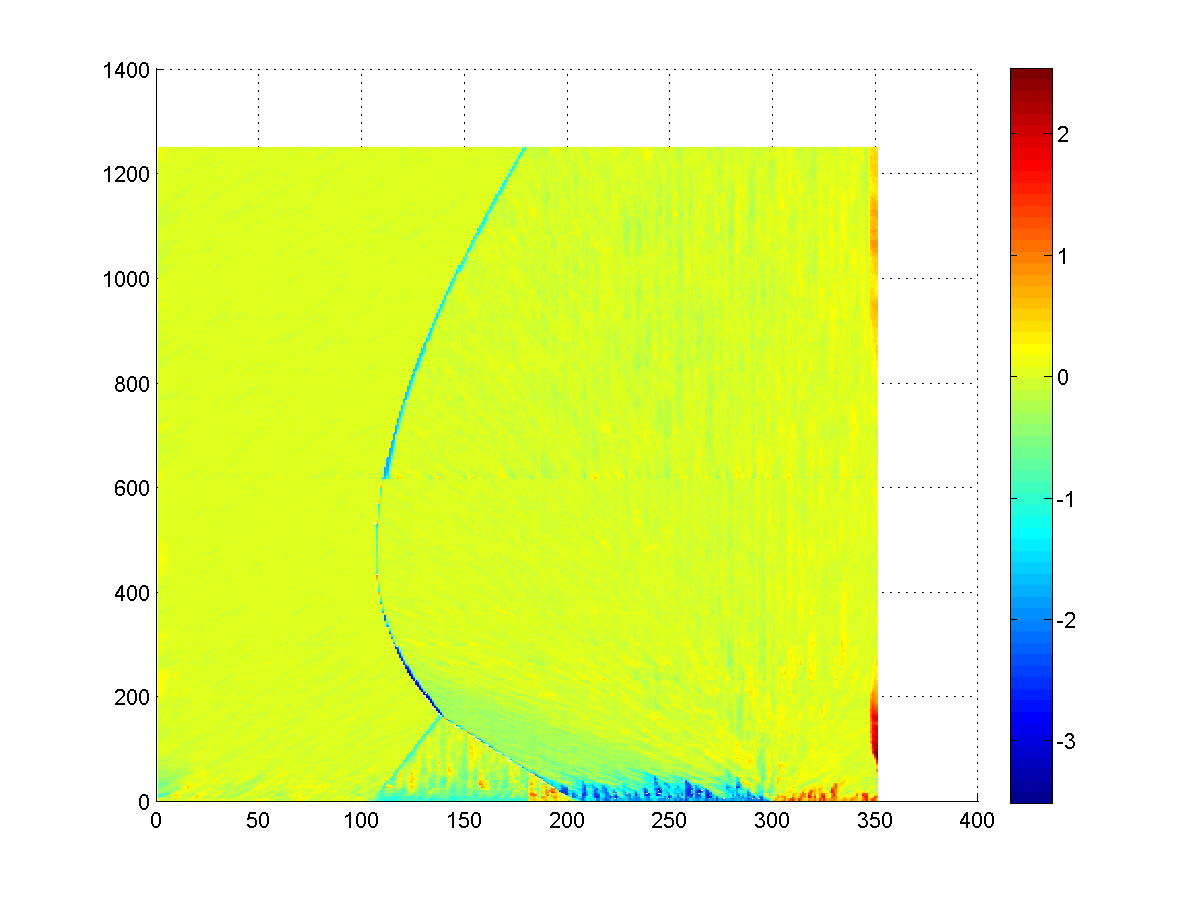
\includegraphics[width = 6cm]{../Simulation_Results/Test_EnKF/Fixed_steps_and_noise_meas_in_stateN_05.png}}
  \subfloat[3D plot]{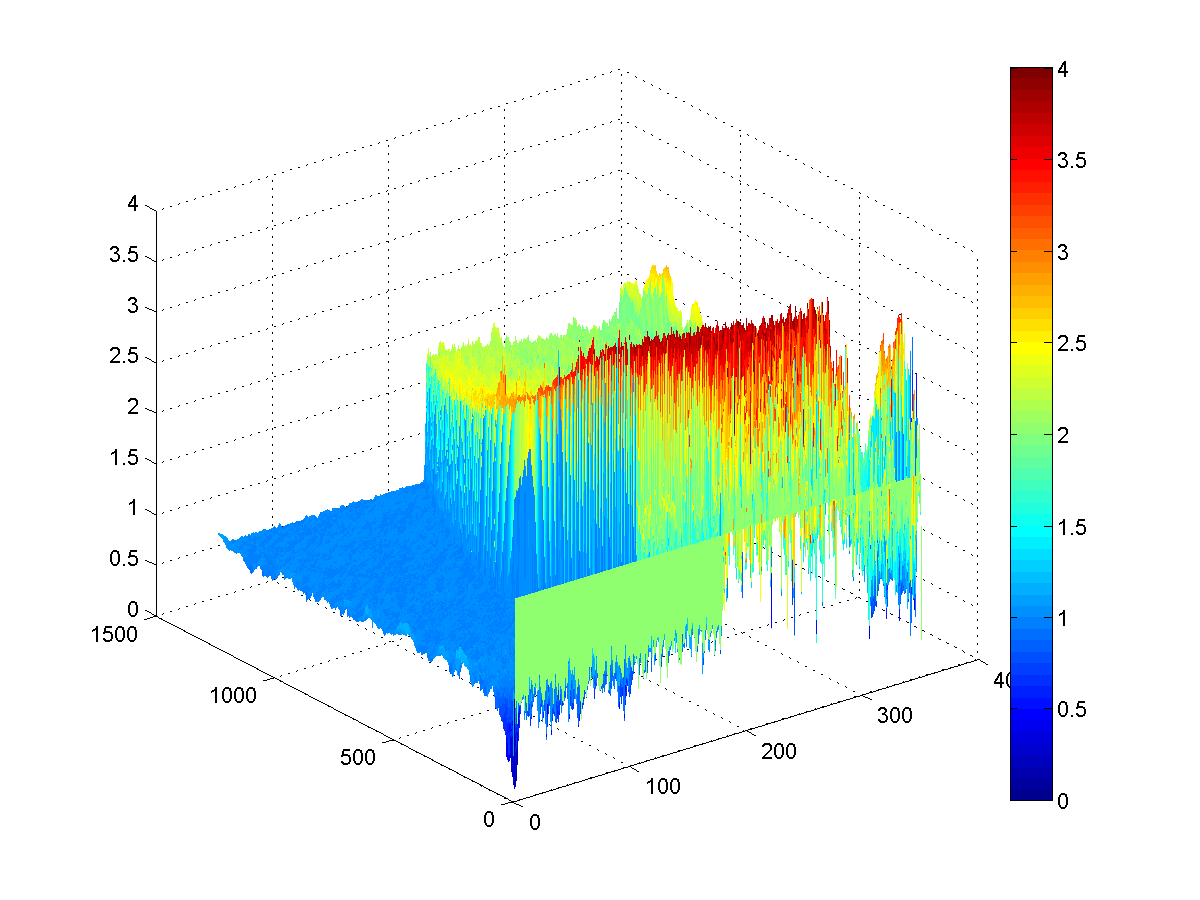
\includegraphics[width = 6cm]{../Simulation_Results/Test_EnKF/Fixed_steps_and_noise_meas_in_stateN_05_3D.png}}
  \caption{Test EnKF, influence of the state noise : 5\%}\label{influence_stateNoise2}
\end{figure}

\begin{figure}
  \centering
  \subfloat[time-space plot]{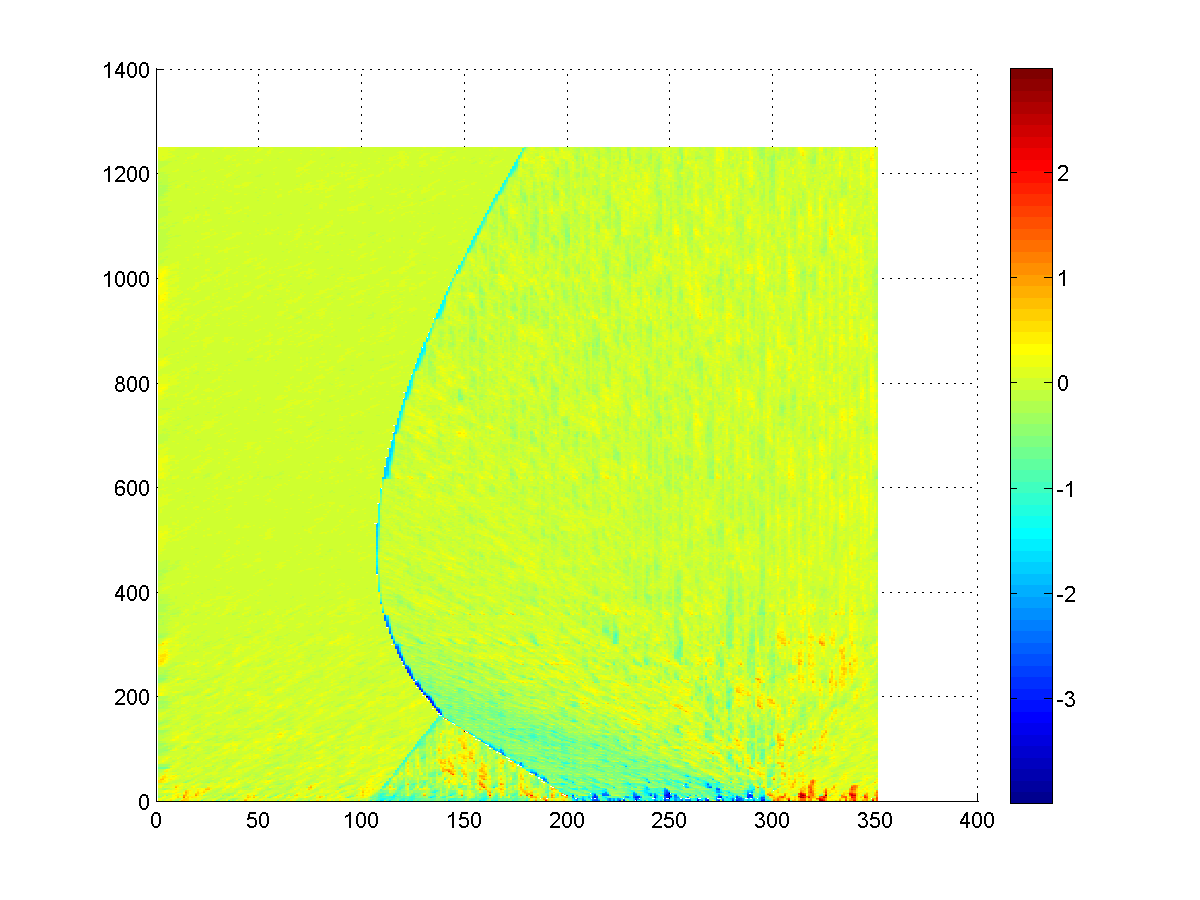
\includegraphics[width = 6cm]{../Simulation_Results/Test_EnKF/Fixed_steps_and_noise_meas_in_stateN_1.png}}
  \subfloat[3D plot]{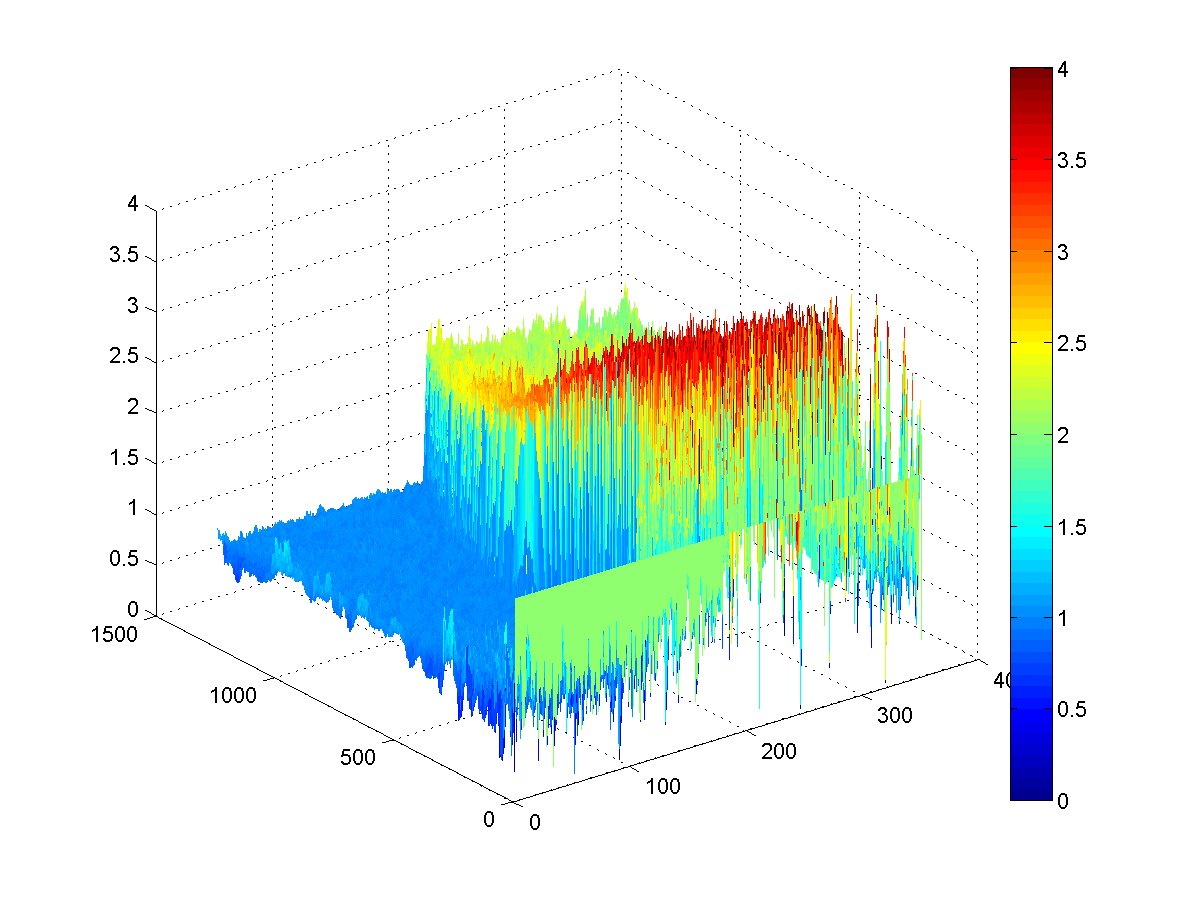
\includegraphics[width = 6cm]{../Simulation_Results/Test_EnKF/Fixed_steps_and_noise_meas_in_stateN_1_3D.png}}
  \caption{Test EnKF, influence of the state noise : 10\%}\label{influence_stateNoise3}
\end{figure}

From the observation of these figures, we can infer that it is better to keep the state noise small to reach a 'smooth' numerical solution with a better 'steady-state'. Although the numerical solution may reach the analytical solution faster with a more significant noise, it is better to keep it small. Indeed, the speed of convergence of the numerical simulation with data assimilation can be improved with a better initial guess of density or a bigger initial noise to generate the ensemble - to 'catch' extreme values of density. As regards the measurements noise, we decided to fix it at 5\%. In a real-life problem, this value would be imposed by sensors properties, and, therefore, this is not a parameter we can tune.  

\bigskip
\paragraph{Modified Forecast}
In our first simulations, before having tuned the value of the state noise, we had trouble obtaining 'smooth' solutions. We realized that the state noise was one of the main reason. Indeed, as we make sure that at each time step the density stay between $0$ and $\rho_{max}$, the addition of a state  noise after the forecast may result in a biased noise. Therefore, we tried another approach in which we also propagate the state noise using the CTM. In other words, Eq(\ref{eq:enkf1}) becomes: 
\begin{equation}
\rho_{f}^{n}(k) =\mathcal{M}(\rho_{a}^{n-1}(k)+\eta^{n}(k))\label{eq:enkf1_modif}
\end{equation}
Finally, it turns out that the results are very similar. The modified EnKF even performs worse. Then, the most important factor, to obtain smooth estimates of density, seems to be the covariance of the state noise itself. The presence of the state noise is necessary but its value needs to be very small so as to obtain nice results. Figures \ref{influence_stateNoise1bis} , \ref{influence_stateNoise2bis} and \ref{influence_stateNoise3bis} show the result of the same simulation as the 3 previous Figures, using, this time, the modified EnKF forecast.
\begin{figure}
  \centering
  \subfloat[time-space plot]{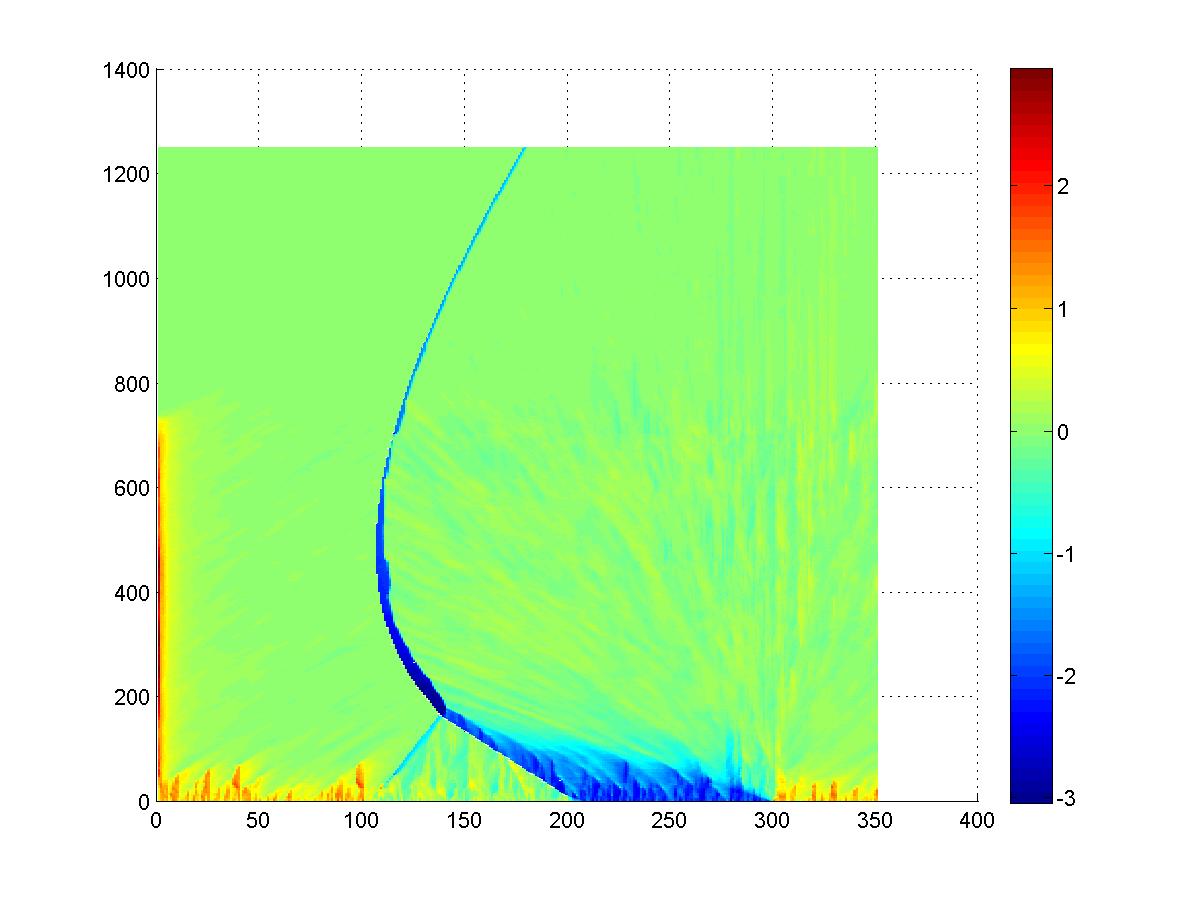
\includegraphics[width = 6cm]{../Simulation_Results/Test_EnKF/Fixed_steps_and_noise_meas_in_stateN_01bis.png}}
  \subfloat[3D plot]{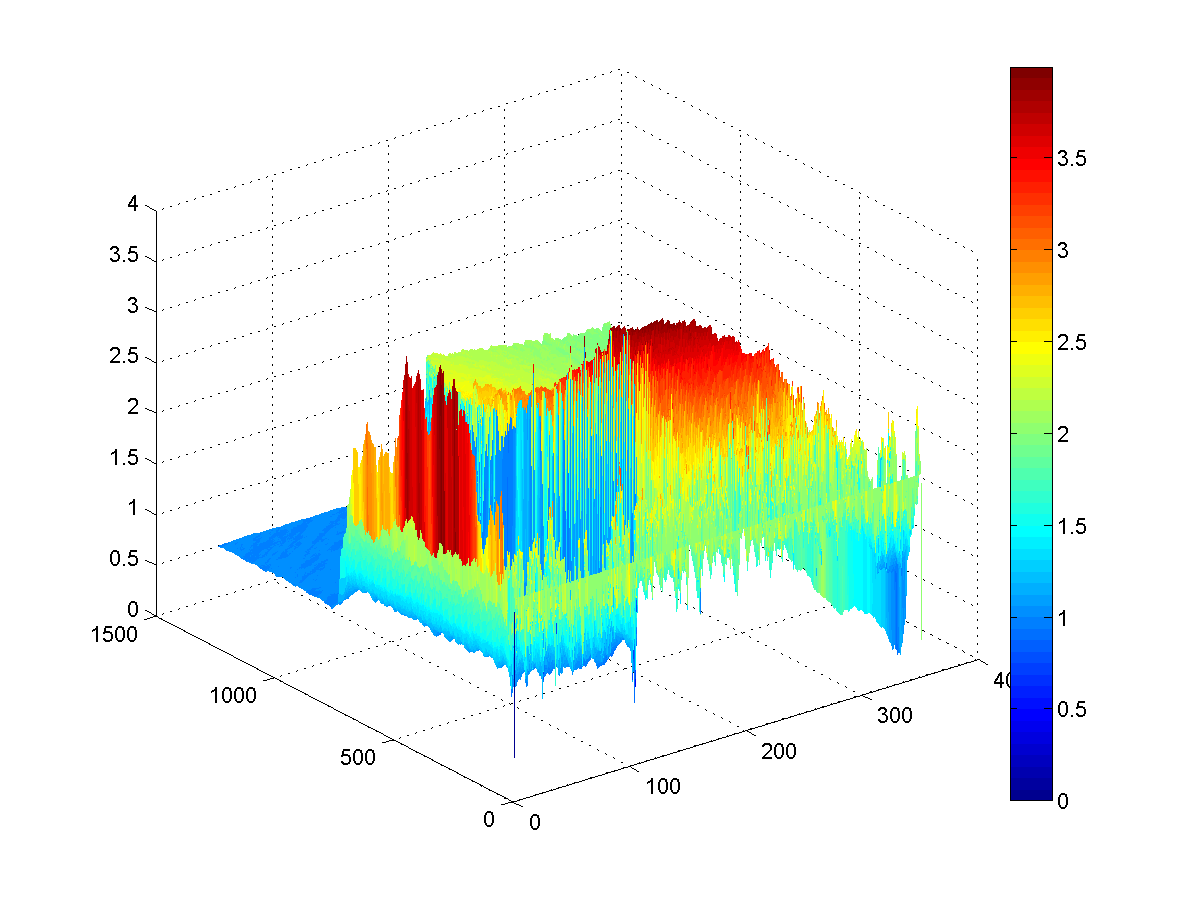
\includegraphics[width = 6cm]{../Simulation_Results/Test_EnKF/Fixed_steps_and_noise_meas_in_stateN_01_3Dbis.png}}
  \caption{Test EnKF modified, influence of the state noise : 1\%}\label{influence_stateNoise1bis}
\end{figure}

\begin{figure}
  \centering
   \subfloat[time-space plot]{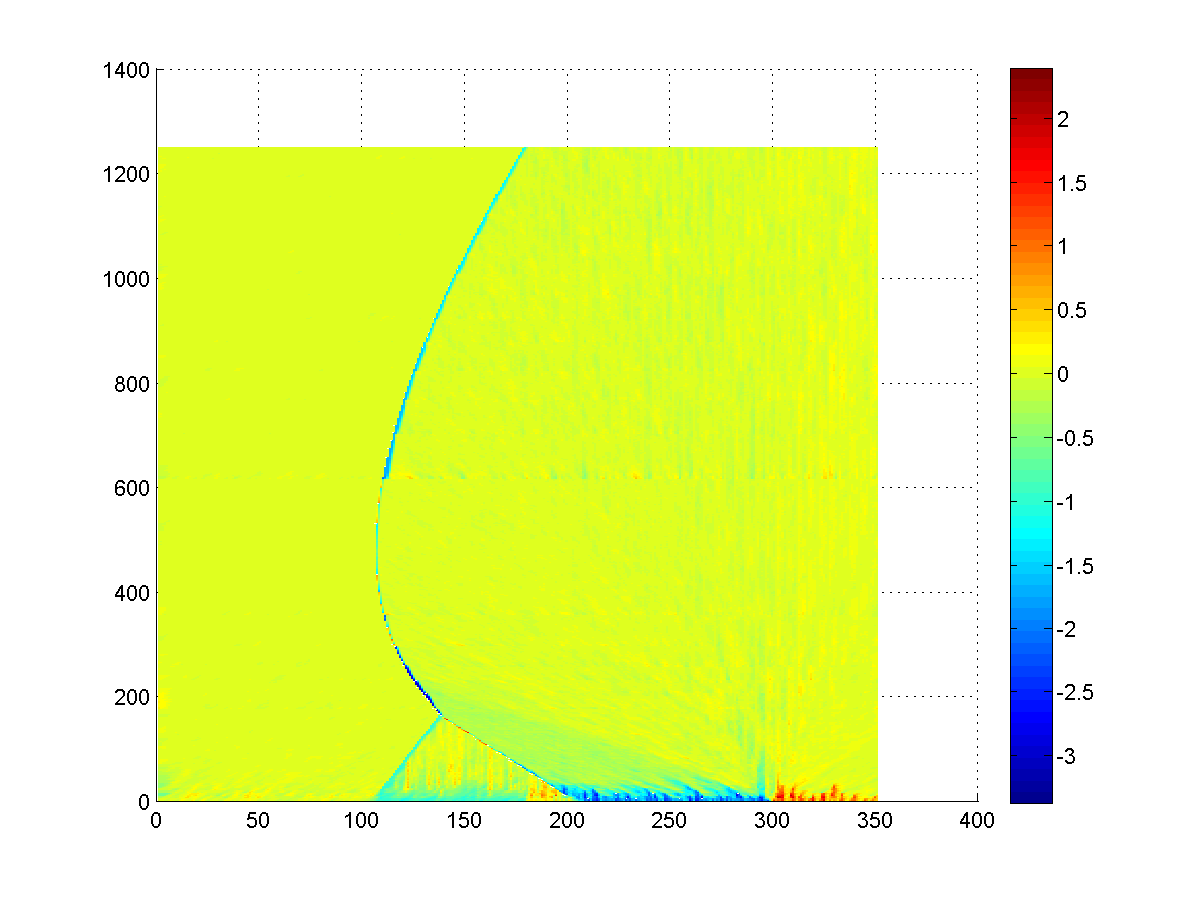
\includegraphics[width = 6cm]{../Simulation_Results/Test_EnKF/Fixed_steps_and_noise_meas_in_stateN_05bis.png}}
  \subfloat[3D plot]{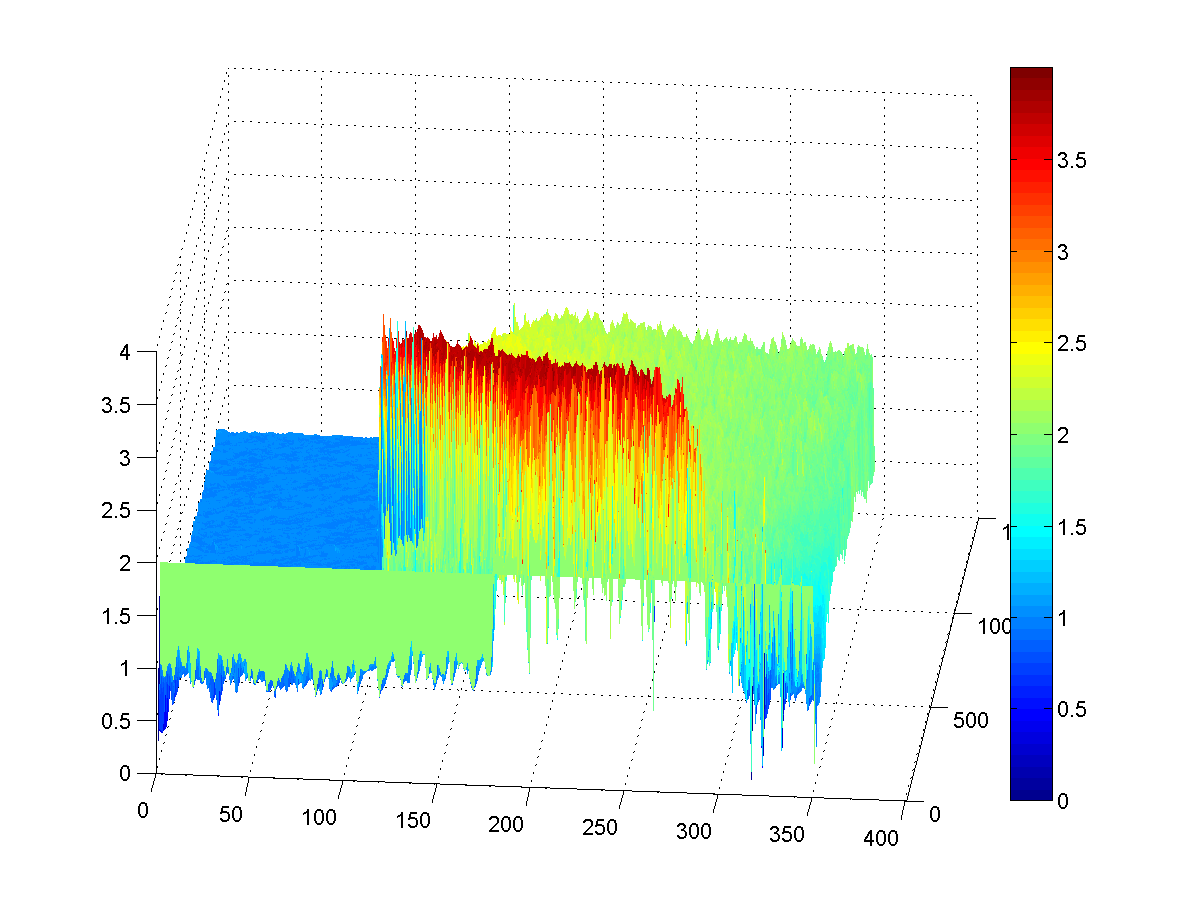
\includegraphics[width = 6cm]{../Simulation_Results/Test_EnKF/Fixed_steps_and_noise_meas_in_stateN_05_3Dbis.png}}
  \caption{Test EnKF modified, influence of the state noise : 5\%}\label{influence_stateNoise2bis}
\end{figure}

\begin{figure}
  \centering
  \subfloat[time-space plot]{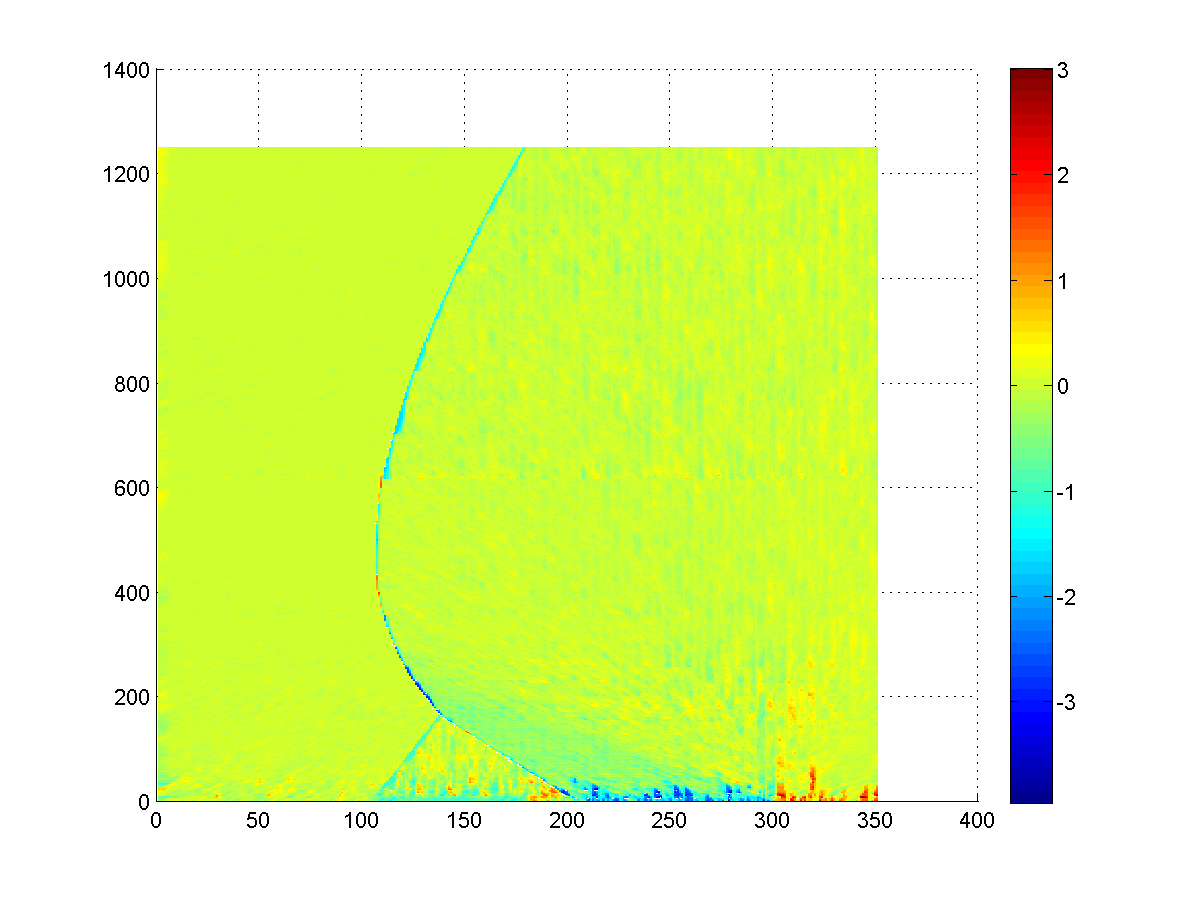
\includegraphics[width = 6cm]{../Simulation_Results/Test_EnKF/Fixed_steps_and_noise_meas_in_stateN_1bis.png}}
  \subfloat[3D plot]{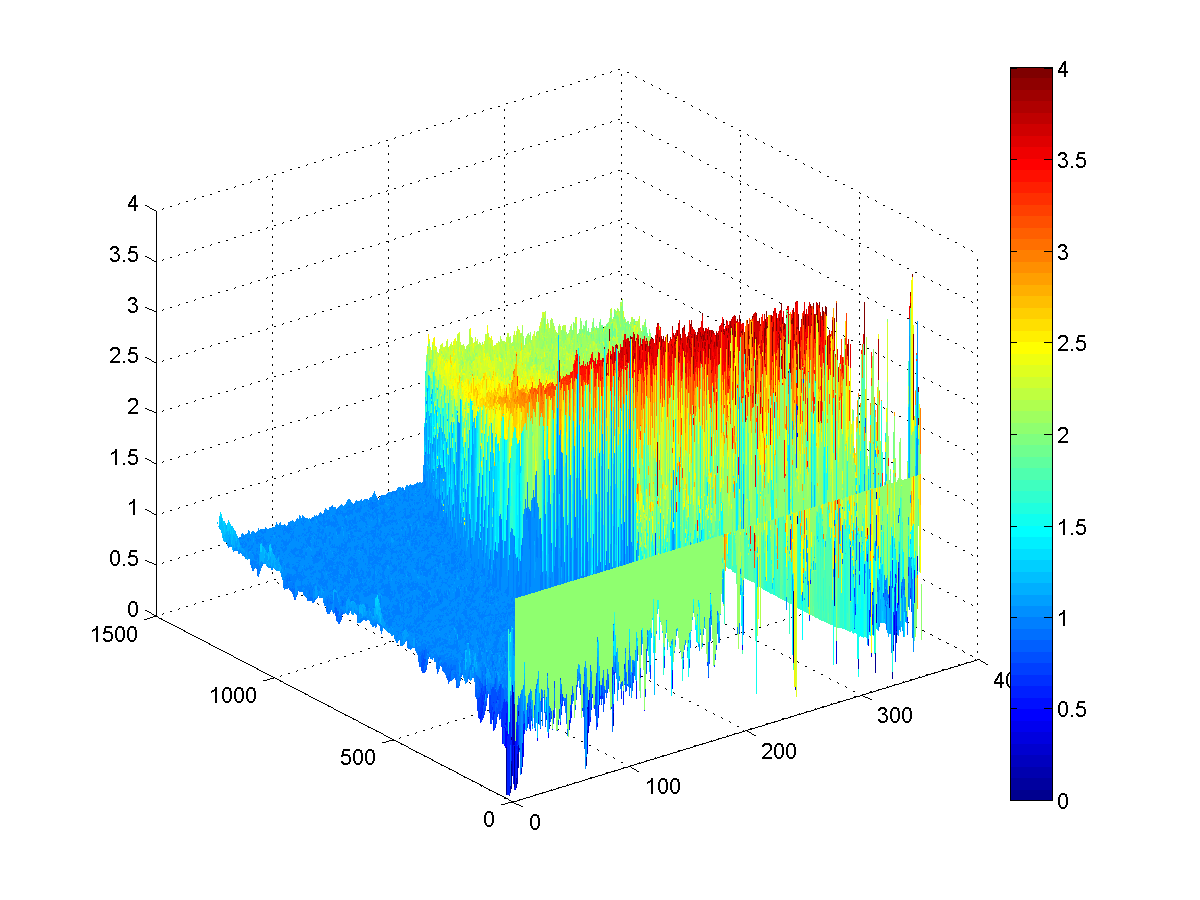
\includegraphics[width = 6cm]{../Simulation_Results/Test_EnKF/Fixed_steps_and_noise_meas_in_stateN_1_3Dbis.png}}
  \caption{Test EnKF modified, influence of the state noise : 10\%}\label{influence_stateNoise3bis}
 \end{figure}
 
 As regards the number of measurements and the frequency at which you get them, there are obvious trade-offs between computation and accuracy. However, for small percentages (in time and space) the EnKF still converges to the analytical. Indeed, Figure \ref{influence_change_percent} shows again the efficiency of the Ensemble Kalman Filter.
 
 \begin{figure}
  \centering
  \subfloat[time-space plot]{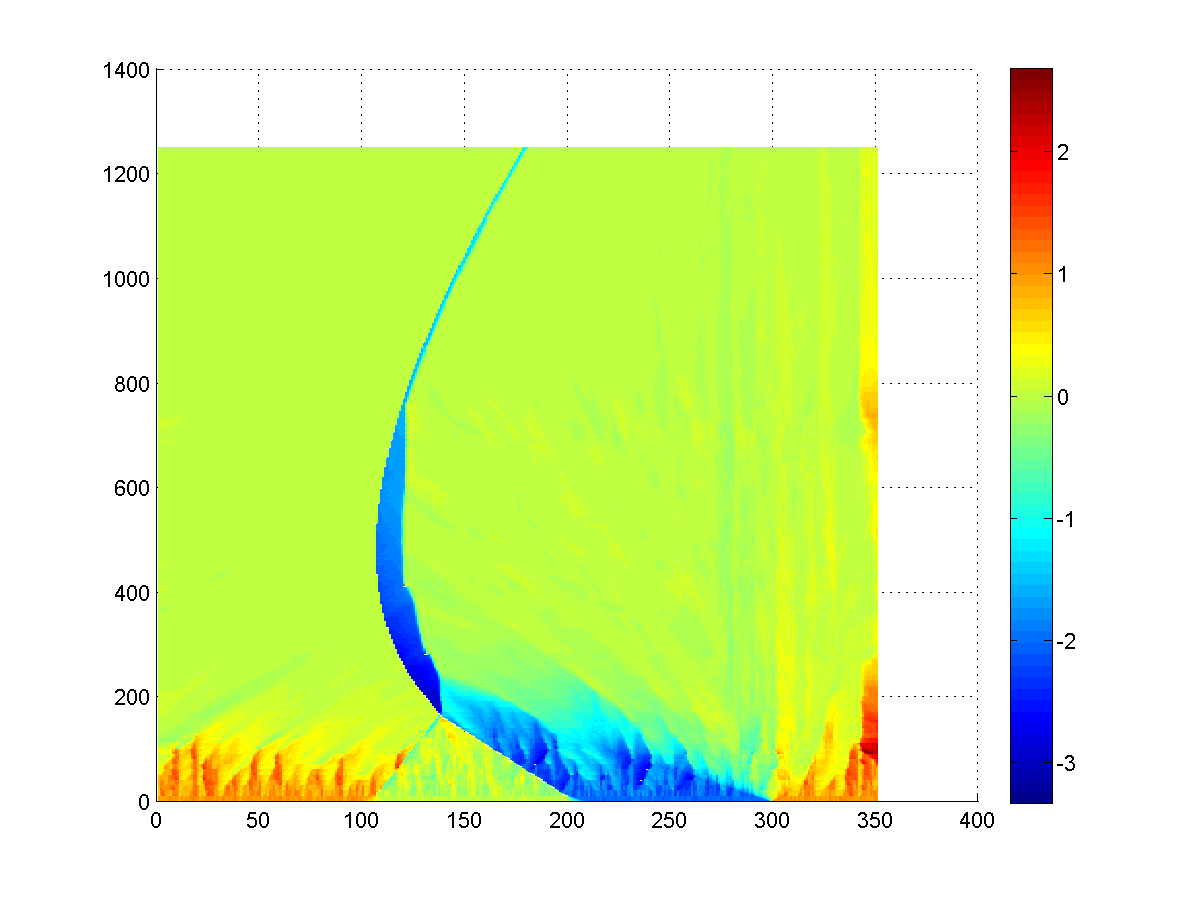
\includegraphics[width = 6cm]{../Simulation_Results/Test_EnKF/Fixed_steps_and_noise_meas_in_inN_01.png}}
  \subfloat[3D plot]{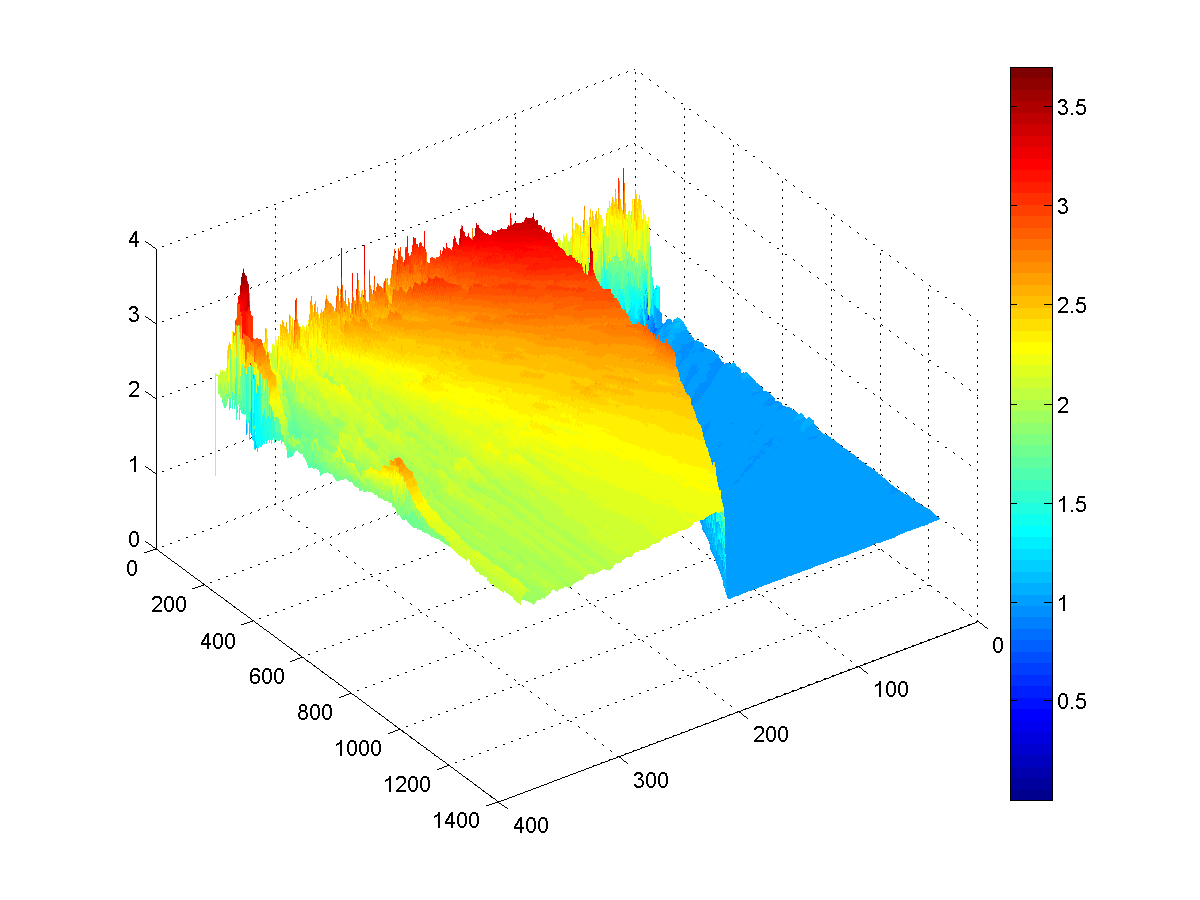
\includegraphics[width = 6cm]{../Simulation_Results/Test_EnKF/Fixed_steps_and_noise_meas_in_inN_01_3D.png}}
  \caption{Test EnKF influence of the quantity of measurements : 10\% in t and x}\label{influence_change_percent}
 \end{figure}
 
\paragraph{Conclusion on the implementation of the EnKF}
From all these observations, it seems like high values of noise - in a reasonable range (<10\%)- enable faster reaction to abrupt changes in density whereas small values guarantee a smoother and more accurate solution after some time. Therefore, for our experiments on real data, we preferred small values of state noise.

\newpage
\section{Bluetooth Validation and Empirical Results \label{sec:val}}
To evaluate the validity of our approach, we use vehicle travel times obtained by Bluetooth sensors. This section details our validation methodology, the Bluetooth data extraction process and the comparison process between our model output and the Bluetooth output.

\subsection{Methodology}

The idea is to compare travel times obtained via Bluetooth sensors on the one hand and via the density map output of our model on the other hand. This density map can be transformed to a velocity map by simply using the inversion formula which is determined by the choice of the fundamental diagram. Let us recall that our traffic estimation model uses traffic counts from loop detectors, which after appropriate filtering enables us to get density data measurements. Because there is no measurable ground truth value for instantaneous point densities, we use travel times obtained via Bluetooth sensors as a proxy. This methodology has been developed as part of the California Center For Innovative Transportation \textit{Hybrid Traffic Data Roadmap project}, in which we were involved as part of our individual research. Figure \ref{fig:dataValFrame} captures the data validation framework.

\begin{figure}
  \centering
  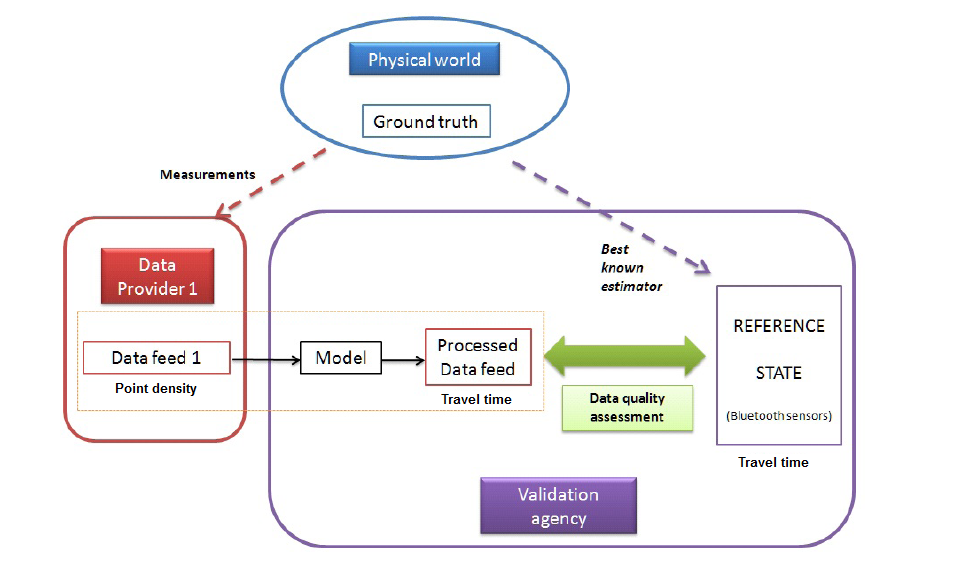
\includegraphics[width = 12cm]{figures/dataValidation.png}                
  \caption{Data Validation Framework}
  \label{fig:dataValFrame}
\end{figure}

 One important aspect of this project was the decision on where to implement this methodology. Three highway segments have been spotted that provide areas with varying historical velocity data and varying sensor penetration rates (the percentage of cars that can be detected) allowing us to validate the performance of the density estimation under different conditions :
\begin{enumerate}
\item Highway I-880 between Winton Avenue and Stevenson Blvd
\item Highway I-15 between Beech Avenue and Bellegrave Avenue
\item Highway I-15 between Los Angeles and Victorville
\end{enumerate}
We will show the results for the first experiment in Section \ref{sec:btResults}.

\bigskip
For more details about the process see \textbf{Validating the use of probe data for highway traffic estimation in the Mobile Millennium highway model using Bluetooth measurements} and \textbf{Implementation of a Reference State using Bluetooth Technology}.

\subsection{Bluetooth data extraction}

\subsubsection{Data feed\label{sec:datafeed}}

Figure \ref{fig:btMap} shows where the Bluetooth sensors are on the map.

\begin{figure}
\centering
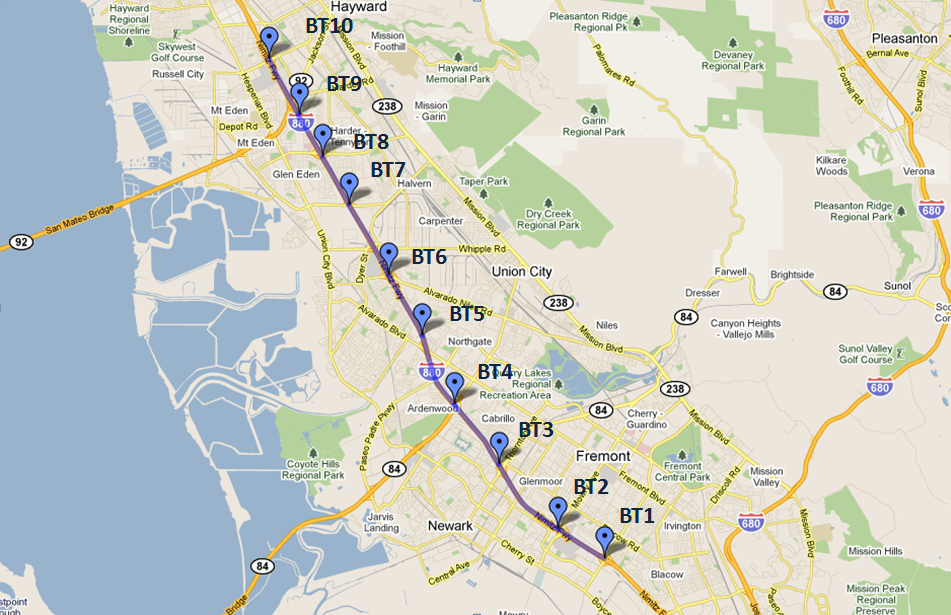
\includegraphics[width=12cm]{figures/btI880Map.png}
    \caption{Map of Bluetooth sensors in Highway I-880}
    \label{fig:btMap}
\end{figure}

\bigskip
A Bluetooth data set is defined by :
\begin{itemize}
\item a number $N$ of Bluetooth readers along with their fixed coordinates.
\item the start and end dates of the experiment.
\item the entire set of sensor's detections of Bluetooth devices.
\end{itemize}
Every day the Bluetooth sensors send emails with zip files containing all their detections for the day with the corresponding time stamp and MAC id. Their average scan duration is 5 seconds.

\subsubsection{Filter \label{sec:filter}}

The first filter’s responsibility is to couple the detections of the same device by consecutive BLUFAX readers. The result of this matching is the list of all the detected trips. But some of these trips may be meaningless (e.g. a car that has been stopped for a while and then starts off again). The second responsibility is then to filter the trips to get rid of the travel time outliers. For this we use an interquartile range filtering technique. Eventually all the trips detected during the validity period are stored in one table.
	
\subsubsection{Travel time comparison\label{sec:comparison}}	
	
The task is basically to compute in parallel the aggregated Bluetooth travel times and highway travel times, and, then, to compute the differences between the two. While doing the analysis one should always keep in mind that there are multiple sources of errors :
\begin{itemize}
\item Model error : The flow theory that gives birth to the LWR equation makes a number of simplifying assumptions that generally do not hold in reality. 
\item Bluetooth measurement errors can alter travel time estimations and therefore result in errors in the validation process
\item Possible bias in Bluetooth equipped vehicles
\end{itemize}  

\subsection{Results \label{sec:btResults}}

In this section we compare the results from our model to the Bluetooth output. To be able to compare these two, we convert the Bluetooth travel times to Bluetooth mean velocities with a 15-minute aggregation period and we convert the densities to velocities using the Greenshields formula $v = v_f (1-\frac{\rho}{\rho_{max}})$. We do this for the first highway segment mentioned in Section \ref{sec:val} on I-880.

\subsubsection{Test on I880}

Figure \ref{fig:comp2FD} shows our results for two different fundamental diagrams. They look really similar and therefore a quantitative analysis would be needed in order to decide on which fundamental diagram is better to use on a large-scale real-time implementation. Figure \ref{fig:compModelBT} shows the accordance between the results of our model and the Bluetooth output. They both show the severe congestion at the evening rush hour on Monday 5th, March 2012. After checking on Google Maps, it actually corresponds to a bottleneck on Highway I880. We can easily see the backward propagation wave which agrees with traffic theoretical principles. The quantitative analysis comparing our results and the Bluetooth travel times is in process and is therefore part of future work.

\begin{figure}
  \begin{center}
    \subfloat[Density output for Greenshields fundamental diagram]{\label{fig:rhoGreenFD}
      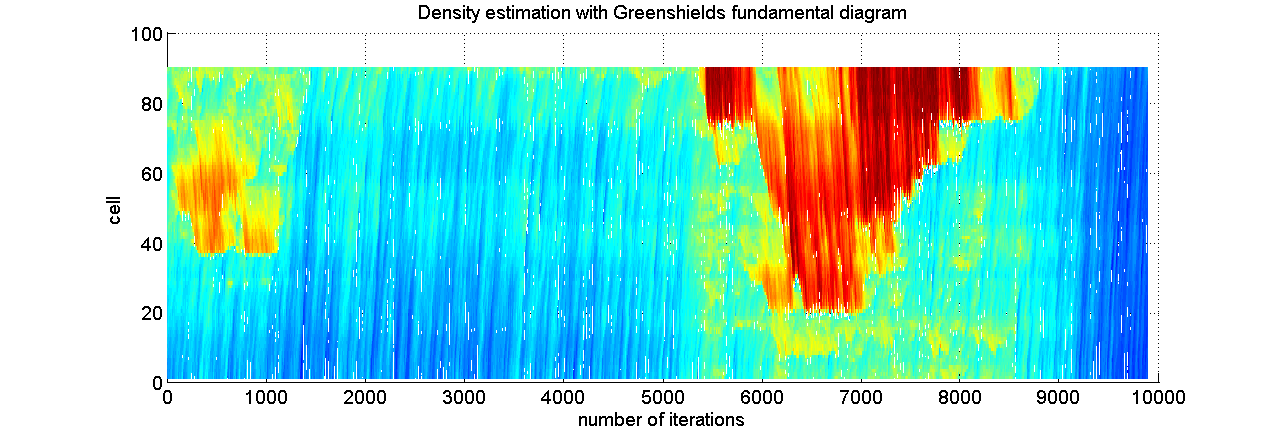
\includegraphics[width=13cm]{figures/Rho_12_3_5_NET_132.png}}
      
    \subfloat[Density output for Daganzo fundamental diagram]{\label{fig:rhoDagFD}
      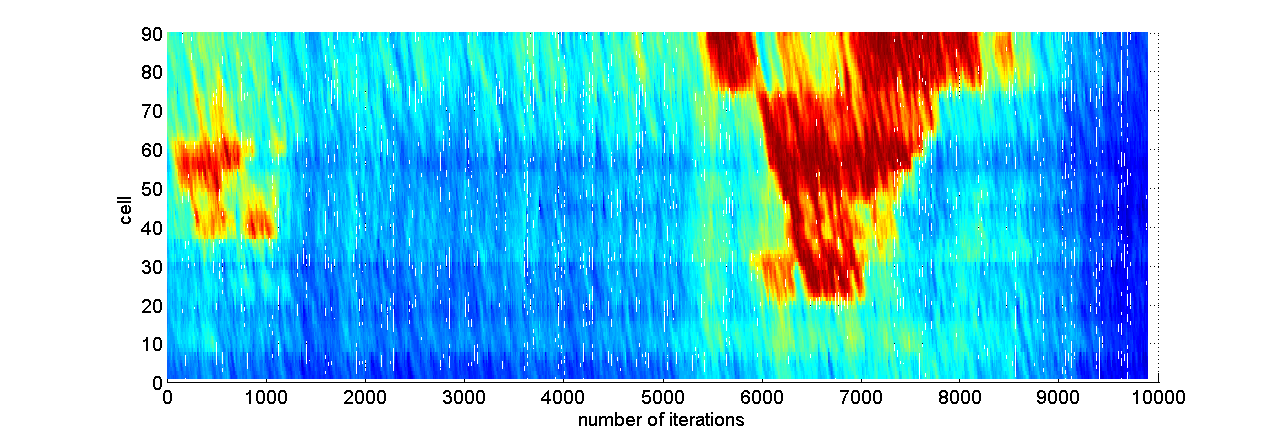
\includegraphics[width=13cm]{figures/Rho_12_3_5_NET_132_DAGANZO.png}}      
  \end{center}
  \caption{Comparison of the output for two fundamental diagrams}
  \label{fig:comp2FD}
\end{figure}

\begin{figure}
  \begin{center}
    \subfloat[Velocity output for Greenshields fundamental diagram]{\label{fig:rhoGreenFD}
      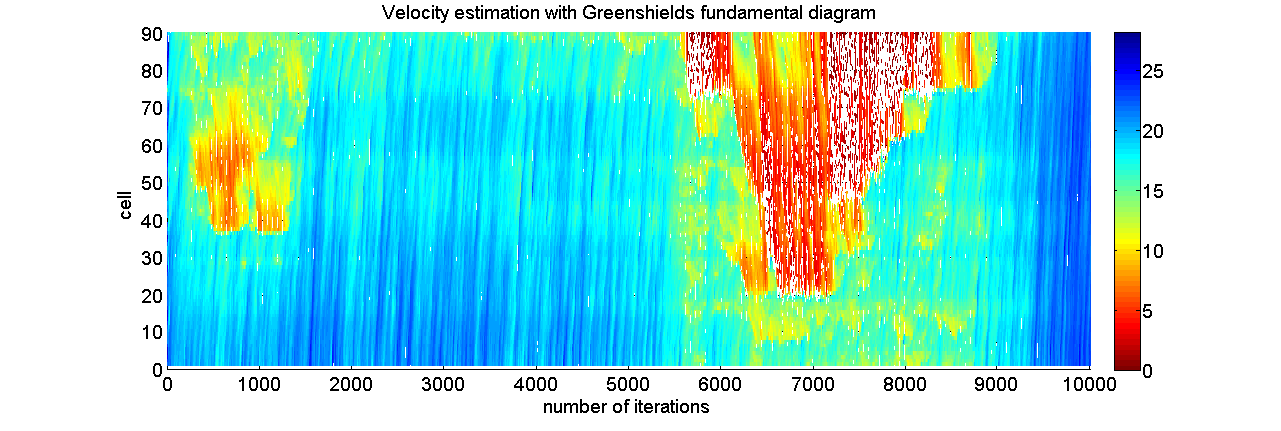
\includegraphics[width=13cm]{figures/Vel_12_3_5_NET_132.png}}
      
    \subfloat[Velocity output for Bluetooth data]{\label{fig:rhoDagFD}
      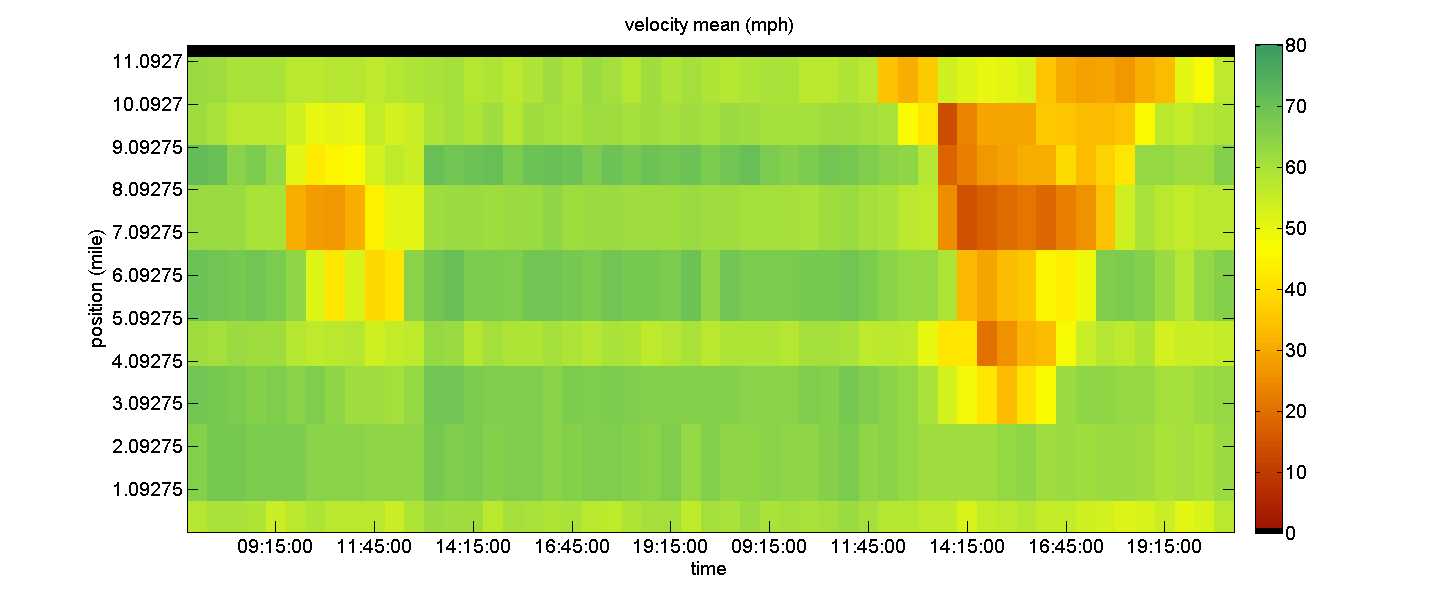
\includegraphics[width=13cm]{figures/BT_12_3_5_A15.png}}
  \end{center}
  \caption{Comparison of model output with Bluetooth output}
  \label{fig:compModelBT}
\end{figure}

\newpage
\section*{Conclusion}

This has been an exciting project showing a nice application of the distributed parameters system theory. The results that we get are really encouraging and we see that the Ensemble Kalman Filter seems to perform well for real density data assimilation. In this report we first introduced the existing traffic estimation theory with density data assimilation. Then we presented our algorithm and its implementation. We showed exhaustive qualitative and quantitative analysis by comparing our results with a known analytical solution. This analysis validated our implementation and provided interesting insights on the relative influences of the involved parameters. Finally we explained our methodology for an experimental validation of the model on real data that were collected on Californian highways and retrieved from the Mobile Millennium database. Once again the results were encouraging and this the reason why we would like to pursue this project in the future. The next steps are the extension of our implementation to road networks as well as a deeper analysis of the results and tuning of all the parameters involoved. We have already developed a script that automatically constructs roads and applies our algorithms, that should enable us to implement large-scale traffic estimation shortly.

\newpage
\bibliography{myBiblio}
\bibliographystyle{plain}

\end{document}